\documentclass[twoside]{book}

% Packages required by doxygen
\usepackage{fixltx2e}
\usepackage{calc}
\usepackage{doxygen}
\usepackage[export]{adjustbox} % also loads graphicx
\usepackage{graphicx}
\usepackage[utf8]{inputenc}
\usepackage{makeidx}
\usepackage{multicol}
\usepackage{multirow}
\PassOptionsToPackage{warn}{textcomp}
\usepackage{textcomp}
\usepackage[nointegrals]{wasysym}
\usepackage[table]{xcolor}

% Font selection
\usepackage[T1]{fontenc}
\usepackage[scaled=.90]{helvet}
\usepackage{courier}
\usepackage{amssymb}
\usepackage{sectsty}
\renewcommand{\familydefault}{\sfdefault}
\allsectionsfont{%
  \fontseries{bc}\selectfont%
  \color{darkgray}%
}
\renewcommand{\DoxyLabelFont}{%
  \fontseries{bc}\selectfont%
  \color{darkgray}%
}
\newcommand{\+}{\discretionary{\mbox{\scriptsize$\hookleftarrow$}}{}{}}

% Page & text layout
\usepackage{geometry}
\geometry{%
  a4paper,%
  top=2.5cm,%
  bottom=2.5cm,%
  left=2.5cm,%
  right=2.5cm%
}
\tolerance=750
\hfuzz=15pt
\hbadness=750
\setlength{\emergencystretch}{15pt}
\setlength{\parindent}{0cm}
\setlength{\parskip}{3ex plus 2ex minus 2ex}
\makeatletter
\renewcommand{\paragraph}{%
  \@startsection{paragraph}{4}{0ex}{-1.0ex}{1.0ex}{%
    \normalfont\normalsize\bfseries\SS@parafont%
  }%
}
\renewcommand{\subparagraph}{%
  \@startsection{subparagraph}{5}{0ex}{-1.0ex}{1.0ex}{%
    \normalfont\normalsize\bfseries\SS@subparafont%
  }%
}
\makeatother

% Headers & footers
\usepackage{fancyhdr}
\pagestyle{fancyplain}
\fancyhead[LE]{\fancyplain{}{\bfseries\thepage}}
\fancyhead[CE]{\fancyplain{}{}}
\fancyhead[RE]{\fancyplain{}{\bfseries\leftmark}}
\fancyhead[LO]{\fancyplain{}{\bfseries\rightmark}}
\fancyhead[CO]{\fancyplain{}{}}
\fancyhead[RO]{\fancyplain{}{\bfseries\thepage}}
\fancyfoot[LE]{\fancyplain{}{}}
\fancyfoot[CE]{\fancyplain{}{}}
\fancyfoot[RE]{\fancyplain{}{\bfseries\scriptsize Generated by Doxygen }}
\fancyfoot[LO]{\fancyplain{}{\bfseries\scriptsize Generated by Doxygen }}
\fancyfoot[CO]{\fancyplain{}{}}
\fancyfoot[RO]{\fancyplain{}{}}
\renewcommand{\footrulewidth}{0.4pt}
\renewcommand{\chaptermark}[1]{%
  \markboth{#1}{}%
}
\renewcommand{\sectionmark}[1]{%
  \markright{\thesection\ #1}%
}

% Indices & bibliography
\usepackage{natbib}
\usepackage[titles]{tocloft}
\setcounter{tocdepth}{3}
\setcounter{secnumdepth}{5}
\makeindex

% Hyperlinks (required, but should be loaded last)
\usepackage{ifpdf}
\ifpdf
  \usepackage[pdftex,pagebackref=true]{hyperref}
\else
  \usepackage[ps2pdf,pagebackref=true]{hyperref}
\fi
\hypersetup{%
  colorlinks=true,%
  linkcolor=blue,%
  citecolor=blue,%
  unicode%
}

% Custom commands
\newcommand{\clearemptydoublepage}{%
  \newpage{\pagestyle{empty}\cleardoublepage}%
}

\usepackage{caption}
\captionsetup{labelsep=space,justification=centering,font={bf},singlelinecheck=off,skip=4pt,position=top}

%===== C O N T E N T S =====

\begin{document}

% Titlepage & ToC
\hypersetup{pageanchor=false,
             bookmarksnumbered=true,
             pdfencoding=unicode
            }
\pagenumbering{alph}
\begin{titlepage}
\vspace*{7cm}
\begin{center}%
{\Large V\+D\+S\+Project \\[1ex]\large 1.\+0 }\\
\vspace*{1cm}
{\large Generated by Doxygen 1.8.13}\\
\end{center}
\end{titlepage}
\clearemptydoublepage
\pagenumbering{roman}
\tableofcontents
\clearemptydoublepage
\pagenumbering{arabic}
\hypersetup{pageanchor=true}

%--- Begin generated contents ---
\chapter{B\+DD package}
\label{index}\hypertarget{index}{}\hypertarget{index_intro_sec}{}\section{Introduction}\label{index_intro_sec}
A package for working with Ordered Binary Decision Diagrams (O\+B\+D\+Ds) is provided.

This package allows to reduce said data structures, obtaining equivalent R\+O\+B\+D\+Ds. In order to do so, the if-\/then-\/else (I\+TE) algorithm is used, together with the corresponding unique and computed tables.\hypertarget{index_used_sec}{}\section{Techniques and tools used}\label{index_used_sec}
This package has been implemented in C++ using C\+Lion as I\+DE. Also, this has been done using Test Driven Develpment (T\+DD), with the tests being implemented using Gtest. Finally, this documentation has been generated using Doxygen.\hypertarget{index_devs_sec}{}\section{Developers}\label{index_devs_sec}
This package has been developed by\+:
\begin{DoxyItemize}
\item Dino Mehmedagić
\item Juan Felipe Vargas Colorado
\item Mateo Vázquez Maceiras 
\end{DoxyItemize}
\chapter{Hierarchical Index}
\section{Class Hierarchy}
This inheritance list is sorted roughly, but not completely, alphabetically\+:\begin{DoxyCompactList}
\item \contentsline{section}{c\+Table\+Val}{\pageref{structcTableVal}}{}
\item \contentsline{section}{Manager\+Interface}{\pageref{classManagerInterface}}{}
\begin{DoxyCompactList}
\item \contentsline{section}{Manager}{\pageref{classManager}}{}
\end{DoxyCompactList}
\item \contentsline{section}{u\+Table\+Val}{\pageref{structuTableVal}}{}
\end{DoxyCompactList}

\chapter{Class Index}
\section{Class List}
Here are the classes, structs, unions and interfaces with brief descriptions\+:\begin{DoxyCompactList}
\item\contentsline{section}{\hyperlink{classClassProject_1_1Manager}{Class\+Project\+::\+Manager} \\*Implements the interface of the B\+DD package }{\pageref{classClassProject_1_1Manager}}{}
\item\contentsline{section}{\hyperlink{classClassProject_1_1ManagerInterface}{Class\+Project\+::\+Manager\+Interface} \\*Defines the implemented interface of the B\+DD package }{\pageref{classClassProject_1_1ManagerInterface}}{}
\item\contentsline{section}{\hyperlink{classClassProject_1_1Reachable}{Class\+Project\+::\+Reachable} \\*Implements the interface of the reachability extension }{\pageref{classClassProject_1_1Reachable}}{}
\item\contentsline{section}{\hyperlink{classClassProject_1_1ReachableInterface}{Class\+Project\+::\+Reachable\+Interface} \\*Defines the implemented interface of the reachability extension }{\pageref{classClassProject_1_1ReachableInterface}}{}
\item\contentsline{section}{\hyperlink{structClassProject_1_1uTableVal}{Class\+Project\+::u\+Table\+Val} \\*Struct used as value in the unique table }{\pageref{structClassProject_1_1uTableVal}}{}
\end{DoxyCompactList}

\chapter{Class Documentation}
\hypertarget{classClassProject_1_1Manager}{}\section{Class\+Project\+:\+:Manager Class Reference}
\label{classClassProject_1_1Manager}\index{Class\+Project\+::\+Manager@{Class\+Project\+::\+Manager}}


Implements the interface of the B\+DD package.  




{\ttfamily \#include $<$Manager.\+h$>$}



Inheritance diagram for Class\+Project\+:\+:Manager\+:
\nopagebreak
\begin{figure}[H]
\begin{center}
\leavevmode
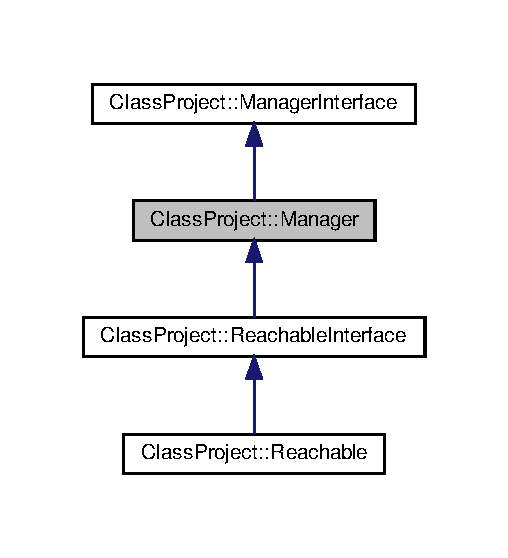
\includegraphics[width=244pt]{classClassProject_1_1Manager__inherit__graph}
\end{center}
\end{figure}


Collaboration diagram for Class\+Project\+:\+:Manager\+:
\nopagebreak
\begin{figure}[H]
\begin{center}
\leavevmode
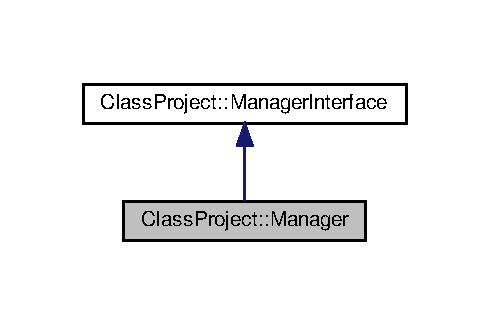
\includegraphics[width=235pt]{classClassProject_1_1Manager__coll__graph}
\end{center}
\end{figure}
\subsection*{Public Member Functions}
\begin{DoxyCompactItemize}
\item 
\hyperlink{classClassProject_1_1Manager_a1658ff9f18e38ccd9cb8b0b371b9c20b}{Manager} ()
\begin{DoxyCompactList}\small\item\em Constructor. \end{DoxyCompactList}\item 
\hyperlink{classClassProject_1_1Manager_a322cad25d7007438b3a043ad02253d29}{$\sim$\+Manager} ()
\item 
const B\+D\+D\+\_\+\+ID \& \hyperlink{classClassProject_1_1Manager_a0c15aff167a7019502b66100c4ec0a33}{True} ()
\item 
const B\+D\+D\+\_\+\+ID \& \hyperlink{classClassProject_1_1Manager_ae9bae01509e6063313024cd85a8eb569}{False} ()
\item 
bool \hyperlink{classClassProject_1_1Manager_a98fe06b67d8114f1404a7b19dddc935b}{is\+Constant} (const B\+D\+D\+\_\+\+ID f)
\item 
bool \hyperlink{classClassProject_1_1Manager_af026f76f68823bb9083f161b5db9e58b}{is\+Variable} (const B\+D\+D\+\_\+\+ID x)
\item 
B\+D\+D\+\_\+\+ID \hyperlink{classClassProject_1_1Manager_a8ddf48759e4e3a5c9e92b07470372b7e}{top\+Var} (const B\+D\+D\+\_\+\+ID f)
\item 
B\+D\+D\+\_\+\+ID \hyperlink{classClassProject_1_1Manager_a9fb480d8af44c75ee2b35b85f7038e68}{create\+Var} (const std\+::string \&label)
\item 
B\+D\+D\+\_\+\+ID \hyperlink{classClassProject_1_1Manager_ab6b8135aadc0a5b91b5c651c4046da05}{ite} (const B\+D\+D\+\_\+\+ID i, const B\+D\+D\+\_\+\+ID t, const B\+D\+D\+\_\+\+ID e)
\item 
B\+D\+D\+\_\+\+ID \hyperlink{classClassProject_1_1Manager_aa2bfdbb0fae8e09b2b766336cdf7ce94}{co\+Factor\+True} (const B\+D\+D\+\_\+\+ID f, B\+D\+D\+\_\+\+ID x)
\item 
B\+D\+D\+\_\+\+ID \hyperlink{classClassProject_1_1Manager_aea635ff0e0ec0cc8b43799f2d18de598}{co\+Factor\+False} (const B\+D\+D\+\_\+\+ID f, B\+D\+D\+\_\+\+ID x)
\item 
B\+D\+D\+\_\+\+ID \hyperlink{classClassProject_1_1Manager_ab2b73e9169e978c45a4ebf9aa3bddef8}{co\+Factor\+True} (const B\+D\+D\+\_\+\+ID f)
\item 
B\+D\+D\+\_\+\+ID \hyperlink{classClassProject_1_1Manager_a3e3d13bac159441b8682338fe6a8bcb2}{co\+Factor\+False} (const B\+D\+D\+\_\+\+ID f)
\item 
B\+D\+D\+\_\+\+ID \hyperlink{classClassProject_1_1Manager_a029fff4ef6650e4fd1f0ff37a69252de}{and2} (const B\+D\+D\+\_\+\+ID a, const B\+D\+D\+\_\+\+ID b)
\item 
B\+D\+D\+\_\+\+ID \hyperlink{classClassProject_1_1Manager_a0f415b7af83a3efb6f7020650e68f1c3}{or2} (const B\+D\+D\+\_\+\+ID a, const B\+D\+D\+\_\+\+ID b)
\item 
B\+D\+D\+\_\+\+ID \hyperlink{classClassProject_1_1Manager_a2582e9a9474189a2710c551548c20c19}{xor2} (const B\+D\+D\+\_\+\+ID a, const B\+D\+D\+\_\+\+ID b)
\item 
B\+D\+D\+\_\+\+ID \hyperlink{classClassProject_1_1Manager_ab53a25ffc83724427725347ed3f9e6ce}{neg} (const B\+D\+D\+\_\+\+ID a)
\item 
B\+D\+D\+\_\+\+ID \hyperlink{classClassProject_1_1Manager_abde082c99a3588ad7e25b620e901e6e0}{nand2} (const B\+D\+D\+\_\+\+ID a, const B\+D\+D\+\_\+\+ID b)
\item 
B\+D\+D\+\_\+\+ID \hyperlink{classClassProject_1_1Manager_a1cbba8dc08a8c1bbabce0b98a8fde3be}{nor2} (const B\+D\+D\+\_\+\+ID a, const B\+D\+D\+\_\+\+ID b)
\item 
std\+::string \hyperlink{classClassProject_1_1Manager_a72e49c79e186bfce423eb554cca28ff2}{get\+Top\+Var\+Name} (const B\+D\+D\+\_\+\+ID \&root)
\item 
void \hyperlink{classClassProject_1_1Manager_a2aefec8f025f8d7417eff8493bcd7f04}{find\+Nodes} (const B\+D\+D\+\_\+\+ID \&root, std\+::set$<$ B\+D\+D\+\_\+\+ID $>$ \&nodes\+\_\+of\+\_\+root)
\item 
void \hyperlink{classClassProject_1_1Manager_abf869470f4d1baffca8a140d3196c2ad}{find\+Vars} (const B\+D\+D\+\_\+\+ID \&root, std\+::set$<$ B\+D\+D\+\_\+\+ID $>$ \&vars\+\_\+of\+\_\+root)
\item 
size\+\_\+t \hyperlink{classClassProject_1_1Manager_a82b10a42ec726d42ea4d2e8bc72a3db9}{unique\+Table\+Size} ()
\item 
\hyperlink{structClassProject_1_1uTableVal}{u\+Table\+Val} $\ast$ \hyperlink{classClassProject_1_1Manager_ac08dabf8fdbc314abf2f9a566089c9c7}{getu\+Table\+Val} (B\+D\+D\+\_\+\+ID id)
\item 
bool \hyperlink{classClassProject_1_1Manager_a8be64b55798d49545a549266ae1e9281}{ctable\+Empty} ()
\item 
B\+D\+D\+\_\+\+ID \hyperlink{classClassProject_1_1Manager_a35b9aaf1d448fdbdc2020b119d729527}{find\+\_\+or\+\_\+add\+\_\+u\+Table} (const B\+D\+D\+\_\+\+ID x, const B\+D\+D\+\_\+\+ID high, const B\+D\+D\+\_\+\+ID low)
\end{DoxyCompactItemize}


\subsection{Detailed Description}
Implements the interface of the B\+DD package. 

\subsection{Constructor \& Destructor Documentation}
\mbox{\Hypertarget{classClassProject_1_1Manager_a1658ff9f18e38ccd9cb8b0b371b9c20b}\label{classClassProject_1_1Manager_a1658ff9f18e38ccd9cb8b0b371b9c20b}} 
\index{Class\+Project\+::\+Manager@{Class\+Project\+::\+Manager}!Manager@{Manager}}
\index{Manager@{Manager}!Class\+Project\+::\+Manager@{Class\+Project\+::\+Manager}}
\subsubsection{\texorpdfstring{Manager()}{Manager()}}
{\footnotesize\ttfamily Manager\+::\+Manager (\begin{DoxyParamCaption}{ }\end{DoxyParamCaption})}



Constructor. 

This constructor creates the unique table to store the values of the R\+O\+B\+DD. It also adds the values of \textquotesingle{}0\textquotesingle{} and \textquotesingle{}1\textquotesingle{} to the table, where the ID of \textquotesingle{}0\textquotesingle{} corresponds to 0 and the ID of \textquotesingle{}1\textquotesingle{} is 1 \mbox{\Hypertarget{classClassProject_1_1Manager_a322cad25d7007438b3a043ad02253d29}\label{classClassProject_1_1Manager_a322cad25d7007438b3a043ad02253d29}} 
\index{Class\+Project\+::\+Manager@{Class\+Project\+::\+Manager}!````~Manager@{$\sim$\+Manager}}
\index{````~Manager@{$\sim$\+Manager}!Class\+Project\+::\+Manager@{Class\+Project\+::\+Manager}}
\subsubsection{\texorpdfstring{$\sim$\+Manager()}{~Manager()}}
{\footnotesize\ttfamily Manager\+::$\sim$\+Manager (\begin{DoxyParamCaption}{ }\end{DoxyParamCaption})}

Destructor 

\subsection{Member Function Documentation}
\mbox{\Hypertarget{classClassProject_1_1Manager_a029fff4ef6650e4fd1f0ff37a69252de}\label{classClassProject_1_1Manager_a029fff4ef6650e4fd1f0ff37a69252de}} 
\index{Class\+Project\+::\+Manager@{Class\+Project\+::\+Manager}!and2@{and2}}
\index{and2@{and2}!Class\+Project\+::\+Manager@{Class\+Project\+::\+Manager}}
\subsubsection{\texorpdfstring{and2()}{and2()}}
{\footnotesize\ttfamily B\+D\+D\+\_\+\+ID Manager\+::and2 (\begin{DoxyParamCaption}\item[{const B\+D\+D\+\_\+\+ID}]{a,  }\item[{const B\+D\+D\+\_\+\+ID}]{b }\end{DoxyParamCaption})\hspace{0.3cm}{\ttfamily [virtual]}}

\begin{DoxyReturn}{Returns}
a B\+DD node that represents the correlating \char`\"{}and\char`\"{} function 
\end{DoxyReturn}


Implements \hyperlink{classClassProject_1_1ManagerInterface_af914326d34a1ed42710f7b11e5baf010}{Class\+Project\+::\+Manager\+Interface}.

\mbox{\Hypertarget{classClassProject_1_1Manager_aea635ff0e0ec0cc8b43799f2d18de598}\label{classClassProject_1_1Manager_aea635ff0e0ec0cc8b43799f2d18de598}} 
\index{Class\+Project\+::\+Manager@{Class\+Project\+::\+Manager}!co\+Factor\+False@{co\+Factor\+False}}
\index{co\+Factor\+False@{co\+Factor\+False}!Class\+Project\+::\+Manager@{Class\+Project\+::\+Manager}}
\subsubsection{\texorpdfstring{co\+Factor\+False()}{coFactorFalse()}\hspace{0.1cm}{\footnotesize\ttfamily [1/2]}}
{\footnotesize\ttfamily B\+D\+D\+\_\+\+ID Manager\+::co\+Factor\+False (\begin{DoxyParamCaption}\item[{const B\+D\+D\+\_\+\+ID}]{f,  }\item[{B\+D\+D\+\_\+\+ID}]{x }\end{DoxyParamCaption})\hspace{0.3cm}{\ttfamily [virtual]}}

\begin{DoxyReturn}{Returns}
the negative cofactor of the function defined by f with respect to function x. 
\end{DoxyReturn}


Implements \hyperlink{classClassProject_1_1ManagerInterface_ad749ef1542c5b23bbbce628d6f666fe4}{Class\+Project\+::\+Manager\+Interface}.

\mbox{\Hypertarget{classClassProject_1_1Manager_a3e3d13bac159441b8682338fe6a8bcb2}\label{classClassProject_1_1Manager_a3e3d13bac159441b8682338fe6a8bcb2}} 
\index{Class\+Project\+::\+Manager@{Class\+Project\+::\+Manager}!co\+Factor\+False@{co\+Factor\+False}}
\index{co\+Factor\+False@{co\+Factor\+False}!Class\+Project\+::\+Manager@{Class\+Project\+::\+Manager}}
\subsubsection{\texorpdfstring{co\+Factor\+False()}{coFactorFalse()}\hspace{0.1cm}{\footnotesize\ttfamily [2/2]}}
{\footnotesize\ttfamily B\+D\+D\+\_\+\+ID Manager\+::co\+Factor\+False (\begin{DoxyParamCaption}\item[{const B\+D\+D\+\_\+\+ID}]{f }\end{DoxyParamCaption})\hspace{0.3cm}{\ttfamily [virtual]}}

\begin{DoxyReturn}{Returns}
the negative cofactor of the function defined by node f. 
\end{DoxyReturn}


Implements \hyperlink{classClassProject_1_1ManagerInterface_a308c99661ad02f407d6f2b0af6230e80}{Class\+Project\+::\+Manager\+Interface}.

\mbox{\Hypertarget{classClassProject_1_1Manager_aa2bfdbb0fae8e09b2b766336cdf7ce94}\label{classClassProject_1_1Manager_aa2bfdbb0fae8e09b2b766336cdf7ce94}} 
\index{Class\+Project\+::\+Manager@{Class\+Project\+::\+Manager}!co\+Factor\+True@{co\+Factor\+True}}
\index{co\+Factor\+True@{co\+Factor\+True}!Class\+Project\+::\+Manager@{Class\+Project\+::\+Manager}}
\subsubsection{\texorpdfstring{co\+Factor\+True()}{coFactorTrue()}\hspace{0.1cm}{\footnotesize\ttfamily [1/2]}}
{\footnotesize\ttfamily B\+D\+D\+\_\+\+ID Manager\+::co\+Factor\+True (\begin{DoxyParamCaption}\item[{const B\+D\+D\+\_\+\+ID}]{f,  }\item[{B\+D\+D\+\_\+\+ID}]{x }\end{DoxyParamCaption})\hspace{0.3cm}{\ttfamily [virtual]}}

\begin{DoxyReturn}{Returns}
the positive cofactor of the function defined by f with respect to function x. 
\end{DoxyReturn}


Implements \hyperlink{classClassProject_1_1ManagerInterface_aab8496a0e551abdad99160e152199f4b}{Class\+Project\+::\+Manager\+Interface}.

\mbox{\Hypertarget{classClassProject_1_1Manager_ab2b73e9169e978c45a4ebf9aa3bddef8}\label{classClassProject_1_1Manager_ab2b73e9169e978c45a4ebf9aa3bddef8}} 
\index{Class\+Project\+::\+Manager@{Class\+Project\+::\+Manager}!co\+Factor\+True@{co\+Factor\+True}}
\index{co\+Factor\+True@{co\+Factor\+True}!Class\+Project\+::\+Manager@{Class\+Project\+::\+Manager}}
\subsubsection{\texorpdfstring{co\+Factor\+True()}{coFactorTrue()}\hspace{0.1cm}{\footnotesize\ttfamily [2/2]}}
{\footnotesize\ttfamily B\+D\+D\+\_\+\+ID Manager\+::co\+Factor\+True (\begin{DoxyParamCaption}\item[{const B\+D\+D\+\_\+\+ID}]{f }\end{DoxyParamCaption})\hspace{0.3cm}{\ttfamily [virtual]}}

\begin{DoxyReturn}{Returns}
the positive cofactor of the function defined by node f. 
\end{DoxyReturn}


Implements \hyperlink{classClassProject_1_1ManagerInterface_a4a1880d2245af9130646232551940949}{Class\+Project\+::\+Manager\+Interface}.

\mbox{\Hypertarget{classClassProject_1_1Manager_a9fb480d8af44c75ee2b35b85f7038e68}\label{classClassProject_1_1Manager_a9fb480d8af44c75ee2b35b85f7038e68}} 
\index{Class\+Project\+::\+Manager@{Class\+Project\+::\+Manager}!create\+Var@{create\+Var}}
\index{create\+Var@{create\+Var}!Class\+Project\+::\+Manager@{Class\+Project\+::\+Manager}}
\subsubsection{\texorpdfstring{create\+Var()}{createVar()}}
{\footnotesize\ttfamily B\+D\+D\+\_\+\+ID Manager\+::create\+Var (\begin{DoxyParamCaption}\item[{const std\+::string \&}]{label }\end{DoxyParamCaption})\hspace{0.3cm}{\ttfamily [virtual]}}

Creates a new variable for the B\+DD. \begin{DoxyReturn}{Returns}
the ID assigned to that variable 
\end{DoxyReturn}


Implements \hyperlink{classClassProject_1_1ManagerInterface_ab101acd3fbe6a5e29973d88f9862b8b4}{Class\+Project\+::\+Manager\+Interface}.

\mbox{\Hypertarget{classClassProject_1_1Manager_a8be64b55798d49545a549266ae1e9281}\label{classClassProject_1_1Manager_a8be64b55798d49545a549266ae1e9281}} 
\index{Class\+Project\+::\+Manager@{Class\+Project\+::\+Manager}!ctable\+Empty@{ctable\+Empty}}
\index{ctable\+Empty@{ctable\+Empty}!Class\+Project\+::\+Manager@{Class\+Project\+::\+Manager}}
\subsubsection{\texorpdfstring{ctable\+Empty()}{ctableEmpty()}}
{\footnotesize\ttfamily bool Manager\+::ctable\+Empty (\begin{DoxyParamCaption}{ }\end{DoxyParamCaption})}

\begin{DoxyReturn}{Returns}
true if the computed table is completely empty 
\end{DoxyReturn}
\mbox{\Hypertarget{classClassProject_1_1Manager_ae9bae01509e6063313024cd85a8eb569}\label{classClassProject_1_1Manager_ae9bae01509e6063313024cd85a8eb569}} 
\index{Class\+Project\+::\+Manager@{Class\+Project\+::\+Manager}!False@{False}}
\index{False@{False}!Class\+Project\+::\+Manager@{Class\+Project\+::\+Manager}}
\subsubsection{\texorpdfstring{False()}{False()}}
{\footnotesize\ttfamily const B\+D\+D\+\_\+\+ID \& Manager\+::\+False (\begin{DoxyParamCaption}{ }\end{DoxyParamCaption})\hspace{0.3cm}{\ttfamily [virtual]}}

\begin{DoxyReturn}{Returns}
the ID of the node representing False. 
\end{DoxyReturn}


Implements \hyperlink{classClassProject_1_1ManagerInterface_a98d18e1bc840fd664af015facfdcf690}{Class\+Project\+::\+Manager\+Interface}.

\mbox{\Hypertarget{classClassProject_1_1Manager_a35b9aaf1d448fdbdc2020b119d729527}\label{classClassProject_1_1Manager_a35b9aaf1d448fdbdc2020b119d729527}} 
\index{Class\+Project\+::\+Manager@{Class\+Project\+::\+Manager}!find\+\_\+or\+\_\+add\+\_\+u\+Table@{find\+\_\+or\+\_\+add\+\_\+u\+Table}}
\index{find\+\_\+or\+\_\+add\+\_\+u\+Table@{find\+\_\+or\+\_\+add\+\_\+u\+Table}!Class\+Project\+::\+Manager@{Class\+Project\+::\+Manager}}
\subsubsection{\texorpdfstring{find\+\_\+or\+\_\+add\+\_\+u\+Table()}{find\_or\_add\_uTable()}}
{\footnotesize\ttfamily B\+D\+D\+\_\+\+ID Manager\+::find\+\_\+or\+\_\+add\+\_\+u\+Table (\begin{DoxyParamCaption}\item[{const B\+D\+D\+\_\+\+ID}]{x,  }\item[{const B\+D\+D\+\_\+\+ID}]{high,  }\item[{const B\+D\+D\+\_\+\+ID}]{low }\end{DoxyParamCaption})}

Compares ite result with unique table and updates if needed \mbox{\Hypertarget{classClassProject_1_1Manager_a2aefec8f025f8d7417eff8493bcd7f04}\label{classClassProject_1_1Manager_a2aefec8f025f8d7417eff8493bcd7f04}} 
\index{Class\+Project\+::\+Manager@{Class\+Project\+::\+Manager}!find\+Nodes@{find\+Nodes}}
\index{find\+Nodes@{find\+Nodes}!Class\+Project\+::\+Manager@{Class\+Project\+::\+Manager}}
\subsubsection{\texorpdfstring{find\+Nodes()}{findNodes()}}
{\footnotesize\ttfamily void Manager\+::find\+Nodes (\begin{DoxyParamCaption}\item[{const B\+D\+D\+\_\+\+ID \&}]{root,  }\item[{std\+::set$<$ B\+D\+D\+\_\+\+ID $>$ \&}]{nodes\+\_\+of\+\_\+root }\end{DoxyParamCaption})\hspace{0.3cm}{\ttfamily [virtual]}}

Fills the set of B\+DD nodes which are reachable from the B\+DD node root (including itself). 

Implements \hyperlink{classClassProject_1_1ManagerInterface_ab460e331ffdb85d4128574b3aae72c1e}{Class\+Project\+::\+Manager\+Interface}.

\mbox{\Hypertarget{classClassProject_1_1Manager_abf869470f4d1baffca8a140d3196c2ad}\label{classClassProject_1_1Manager_abf869470f4d1baffca8a140d3196c2ad}} 
\index{Class\+Project\+::\+Manager@{Class\+Project\+::\+Manager}!find\+Vars@{find\+Vars}}
\index{find\+Vars@{find\+Vars}!Class\+Project\+::\+Manager@{Class\+Project\+::\+Manager}}
\subsubsection{\texorpdfstring{find\+Vars()}{findVars()}}
{\footnotesize\ttfamily void Manager\+::find\+Vars (\begin{DoxyParamCaption}\item[{const B\+D\+D\+\_\+\+ID \&}]{root,  }\item[{std\+::set$<$ B\+D\+D\+\_\+\+ID $>$ \&}]{vars\+\_\+of\+\_\+root }\end{DoxyParamCaption})\hspace{0.3cm}{\ttfamily [virtual]}}

Fills the set with variables which are either top variable of the B\+DD node root or the reachable nodes from root. 

Implements \hyperlink{classClassProject_1_1ManagerInterface_ab94feabca2125d334e542e502ae0186d}{Class\+Project\+::\+Manager\+Interface}.

\mbox{\Hypertarget{classClassProject_1_1Manager_a72e49c79e186bfce423eb554cca28ff2}\label{classClassProject_1_1Manager_a72e49c79e186bfce423eb554cca28ff2}} 
\index{Class\+Project\+::\+Manager@{Class\+Project\+::\+Manager}!get\+Top\+Var\+Name@{get\+Top\+Var\+Name}}
\index{get\+Top\+Var\+Name@{get\+Top\+Var\+Name}!Class\+Project\+::\+Manager@{Class\+Project\+::\+Manager}}
\subsubsection{\texorpdfstring{get\+Top\+Var\+Name()}{getTopVarName()}}
{\footnotesize\ttfamily std\+::string Manager\+::get\+Top\+Var\+Name (\begin{DoxyParamCaption}\item[{const B\+D\+D\+\_\+\+ID \&}]{root }\end{DoxyParamCaption})\hspace{0.3cm}{\ttfamily [virtual]}}

\begin{DoxyReturn}{Returns}
the name of top variable of the B\+DD node root 
\end{DoxyReturn}


Implements \hyperlink{classClassProject_1_1ManagerInterface_afde45b2065361dfa6e61c1c7bc3fc1b4}{Class\+Project\+::\+Manager\+Interface}.

\mbox{\Hypertarget{classClassProject_1_1Manager_ac08dabf8fdbc314abf2f9a566089c9c7}\label{classClassProject_1_1Manager_ac08dabf8fdbc314abf2f9a566089c9c7}} 
\index{Class\+Project\+::\+Manager@{Class\+Project\+::\+Manager}!getu\+Table\+Val@{getu\+Table\+Val}}
\index{getu\+Table\+Val@{getu\+Table\+Val}!Class\+Project\+::\+Manager@{Class\+Project\+::\+Manager}}
\subsubsection{\texorpdfstring{getu\+Table\+Val()}{getuTableVal()}}
{\footnotesize\ttfamily \hyperlink{structClassProject_1_1uTableVal}{u\+Table\+Val} $\ast$ Manager\+::getu\+Table\+Val (\begin{DoxyParamCaption}\item[{B\+D\+D\+\_\+\+ID}]{id }\end{DoxyParamCaption})}

Implementation of local functions to manipulate tables \begin{DoxyReturn}{Returns}
an entry from the uniq\+Table 
\end{DoxyReturn}
\mbox{\Hypertarget{classClassProject_1_1Manager_a98fe06b67d8114f1404a7b19dddc935b}\label{classClassProject_1_1Manager_a98fe06b67d8114f1404a7b19dddc935b}} 
\index{Class\+Project\+::\+Manager@{Class\+Project\+::\+Manager}!is\+Constant@{is\+Constant}}
\index{is\+Constant@{is\+Constant}!Class\+Project\+::\+Manager@{Class\+Project\+::\+Manager}}
\subsubsection{\texorpdfstring{is\+Constant()}{isConstant()}}
{\footnotesize\ttfamily bool Manager\+::is\+Constant (\begin{DoxyParamCaption}\item[{const B\+D\+D\+\_\+\+ID}]{f }\end{DoxyParamCaption})\hspace{0.3cm}{\ttfamily [virtual]}}

\begin{DoxyReturn}{Returns}
true if x is a leaf node. 
\end{DoxyReturn}


Implements \hyperlink{classClassProject_1_1ManagerInterface_a0edd879f6ecae7bc5f84a2d55373d977}{Class\+Project\+::\+Manager\+Interface}.

\mbox{\Hypertarget{classClassProject_1_1Manager_af026f76f68823bb9083f161b5db9e58b}\label{classClassProject_1_1Manager_af026f76f68823bb9083f161b5db9e58b}} 
\index{Class\+Project\+::\+Manager@{Class\+Project\+::\+Manager}!is\+Variable@{is\+Variable}}
\index{is\+Variable@{is\+Variable}!Class\+Project\+::\+Manager@{Class\+Project\+::\+Manager}}
\subsubsection{\texorpdfstring{is\+Variable()}{isVariable()}}
{\footnotesize\ttfamily bool Manager\+::is\+Variable (\begin{DoxyParamCaption}\item[{const B\+D\+D\+\_\+\+ID}]{x }\end{DoxyParamCaption})\hspace{0.3cm}{\ttfamily [virtual]}}

\begin{DoxyReturn}{Returns}
true if x is a variable. 
\end{DoxyReturn}


Implements \hyperlink{classClassProject_1_1ManagerInterface_a6eaaec7cbf8826198e490313ccb8f22a}{Class\+Project\+::\+Manager\+Interface}.

\mbox{\Hypertarget{classClassProject_1_1Manager_ab6b8135aadc0a5b91b5c651c4046da05}\label{classClassProject_1_1Manager_ab6b8135aadc0a5b91b5c651c4046da05}} 
\index{Class\+Project\+::\+Manager@{Class\+Project\+::\+Manager}!ite@{ite}}
\index{ite@{ite}!Class\+Project\+::\+Manager@{Class\+Project\+::\+Manager}}
\subsubsection{\texorpdfstring{ite()}{ite()}}
{\footnotesize\ttfamily B\+D\+D\+\_\+\+ID Manager\+::ite (\begin{DoxyParamCaption}\item[{const B\+D\+D\+\_\+\+ID}]{i,  }\item[{const B\+D\+D\+\_\+\+ID}]{t,  }\item[{const B\+D\+D\+\_\+\+ID}]{e }\end{DoxyParamCaption})\hspace{0.3cm}{\ttfamily [virtual]}}

Implements the if-\/then-\/else algorithm. \begin{DoxyReturn}{Returns}
the new node ID that represents the I\+TE. 
\end{DoxyReturn}
ite(1, f, g) = f

ite(0, g, f) = f

ite(f, 1, 0) = f 

Implements \hyperlink{classClassProject_1_1ManagerInterface_a6ea8f9482d86afb4128c52328d9ec11c}{Class\+Project\+::\+Manager\+Interface}.

\mbox{\Hypertarget{classClassProject_1_1Manager_abde082c99a3588ad7e25b620e901e6e0}\label{classClassProject_1_1Manager_abde082c99a3588ad7e25b620e901e6e0}} 
\index{Class\+Project\+::\+Manager@{Class\+Project\+::\+Manager}!nand2@{nand2}}
\index{nand2@{nand2}!Class\+Project\+::\+Manager@{Class\+Project\+::\+Manager}}
\subsubsection{\texorpdfstring{nand2()}{nand2()}}
{\footnotesize\ttfamily B\+D\+D\+\_\+\+ID Manager\+::nand2 (\begin{DoxyParamCaption}\item[{const B\+D\+D\+\_\+\+ID}]{a,  }\item[{const B\+D\+D\+\_\+\+ID}]{b }\end{DoxyParamCaption})\hspace{0.3cm}{\ttfamily [virtual]}}

\begin{DoxyReturn}{Returns}
a B\+DD node that represents the correlating \char`\"{}nand\char`\"{} function 
\end{DoxyReturn}


Implements \hyperlink{classClassProject_1_1ManagerInterface_aaf6e357d680613e449d3ea958c9abba1}{Class\+Project\+::\+Manager\+Interface}.

\mbox{\Hypertarget{classClassProject_1_1Manager_ab53a25ffc83724427725347ed3f9e6ce}\label{classClassProject_1_1Manager_ab53a25ffc83724427725347ed3f9e6ce}} 
\index{Class\+Project\+::\+Manager@{Class\+Project\+::\+Manager}!neg@{neg}}
\index{neg@{neg}!Class\+Project\+::\+Manager@{Class\+Project\+::\+Manager}}
\subsubsection{\texorpdfstring{neg()}{neg()}}
{\footnotesize\ttfamily B\+D\+D\+\_\+\+ID Manager\+::neg (\begin{DoxyParamCaption}\item[{const B\+D\+D\+\_\+\+ID}]{a }\end{DoxyParamCaption})\hspace{0.3cm}{\ttfamily [virtual]}}

\begin{DoxyReturn}{Returns}
a B\+DD node that represents the correlating \char`\"{}neg\char`\"{} function 
\end{DoxyReturn}


Implements \hyperlink{classClassProject_1_1ManagerInterface_a57d34af3121dcf5366d22ecf792f05a0}{Class\+Project\+::\+Manager\+Interface}.

\mbox{\Hypertarget{classClassProject_1_1Manager_a1cbba8dc08a8c1bbabce0b98a8fde3be}\label{classClassProject_1_1Manager_a1cbba8dc08a8c1bbabce0b98a8fde3be}} 
\index{Class\+Project\+::\+Manager@{Class\+Project\+::\+Manager}!nor2@{nor2}}
\index{nor2@{nor2}!Class\+Project\+::\+Manager@{Class\+Project\+::\+Manager}}
\subsubsection{\texorpdfstring{nor2()}{nor2()}}
{\footnotesize\ttfamily B\+D\+D\+\_\+\+ID Manager\+::nor2 (\begin{DoxyParamCaption}\item[{const B\+D\+D\+\_\+\+ID}]{a,  }\item[{const B\+D\+D\+\_\+\+ID}]{b }\end{DoxyParamCaption})\hspace{0.3cm}{\ttfamily [virtual]}}

\begin{DoxyReturn}{Returns}
a B\+DD node that represents the correlating \char`\"{}nor\char`\"{} function 
\end{DoxyReturn}


Implements \hyperlink{classClassProject_1_1ManagerInterface_a312d9865eae2d6355e17855cba78bc78}{Class\+Project\+::\+Manager\+Interface}.

\mbox{\Hypertarget{classClassProject_1_1Manager_a0f415b7af83a3efb6f7020650e68f1c3}\label{classClassProject_1_1Manager_a0f415b7af83a3efb6f7020650e68f1c3}} 
\index{Class\+Project\+::\+Manager@{Class\+Project\+::\+Manager}!or2@{or2}}
\index{or2@{or2}!Class\+Project\+::\+Manager@{Class\+Project\+::\+Manager}}
\subsubsection{\texorpdfstring{or2()}{or2()}}
{\footnotesize\ttfamily B\+D\+D\+\_\+\+ID Manager\+::or2 (\begin{DoxyParamCaption}\item[{const B\+D\+D\+\_\+\+ID}]{a,  }\item[{const B\+D\+D\+\_\+\+ID}]{b }\end{DoxyParamCaption})\hspace{0.3cm}{\ttfamily [virtual]}}

\begin{DoxyReturn}{Returns}
a B\+DD node that represents the correlating \char`\"{}or\char`\"{} function 
\end{DoxyReturn}


Implements \hyperlink{classClassProject_1_1ManagerInterface_a8dbfde761b1e94d1f222b4d27f3c6fbc}{Class\+Project\+::\+Manager\+Interface}.

\mbox{\Hypertarget{classClassProject_1_1Manager_a8ddf48759e4e3a5c9e92b07470372b7e}\label{classClassProject_1_1Manager_a8ddf48759e4e3a5c9e92b07470372b7e}} 
\index{Class\+Project\+::\+Manager@{Class\+Project\+::\+Manager}!top\+Var@{top\+Var}}
\index{top\+Var@{top\+Var}!Class\+Project\+::\+Manager@{Class\+Project\+::\+Manager}}
\subsubsection{\texorpdfstring{top\+Var()}{topVar()}}
{\footnotesize\ttfamily B\+D\+D\+\_\+\+ID Manager\+::top\+Var (\begin{DoxyParamCaption}\item[{const B\+D\+D\+\_\+\+ID}]{f }\end{DoxyParamCaption})\hspace{0.3cm}{\ttfamily [virtual]}}

\begin{DoxyReturn}{Returns}
the ID of top variable of the B\+DD node f 
\end{DoxyReturn}


Implements \hyperlink{classClassProject_1_1ManagerInterface_ae2c645f859bcc7be3376d478f01eb045}{Class\+Project\+::\+Manager\+Interface}.

\mbox{\Hypertarget{classClassProject_1_1Manager_a0c15aff167a7019502b66100c4ec0a33}\label{classClassProject_1_1Manager_a0c15aff167a7019502b66100c4ec0a33}} 
\index{Class\+Project\+::\+Manager@{Class\+Project\+::\+Manager}!True@{True}}
\index{True@{True}!Class\+Project\+::\+Manager@{Class\+Project\+::\+Manager}}
\subsubsection{\texorpdfstring{True()}{True()}}
{\footnotesize\ttfamily const B\+D\+D\+\_\+\+ID \& Manager\+::\+True (\begin{DoxyParamCaption}{ }\end{DoxyParamCaption})\hspace{0.3cm}{\ttfamily [virtual]}}

Implementation of virtual functions from Class \hyperlink{classClassProject_1_1ManagerInterface}{Manager\+Interface} \begin{DoxyReturn}{Returns}
the ID of the node representing True. 
\end{DoxyReturn}


Implements \hyperlink{classClassProject_1_1ManagerInterface_a104d0e8bcbd81eb501b66db6e24d1f63}{Class\+Project\+::\+Manager\+Interface}.

\mbox{\Hypertarget{classClassProject_1_1Manager_a82b10a42ec726d42ea4d2e8bc72a3db9}\label{classClassProject_1_1Manager_a82b10a42ec726d42ea4d2e8bc72a3db9}} 
\index{Class\+Project\+::\+Manager@{Class\+Project\+::\+Manager}!unique\+Table\+Size@{unique\+Table\+Size}}
\index{unique\+Table\+Size@{unique\+Table\+Size}!Class\+Project\+::\+Manager@{Class\+Project\+::\+Manager}}
\subsubsection{\texorpdfstring{unique\+Table\+Size()}{uniqueTableSize()}}
{\footnotesize\ttfamily size\+\_\+t Manager\+::unique\+Table\+Size (\begin{DoxyParamCaption}{ }\end{DoxyParamCaption})\hspace{0.3cm}{\ttfamily [virtual]}}

\begin{DoxyReturn}{Returns}
the number of the nodes currently exist in the unique table of the \hyperlink{classClassProject_1_1Manager}{Manager} class. 
\end{DoxyReturn}


Implements \hyperlink{classClassProject_1_1ManagerInterface_a85cac80444b26e5b80eb96b9f1231c0e}{Class\+Project\+::\+Manager\+Interface}.

\mbox{\Hypertarget{classClassProject_1_1Manager_a2582e9a9474189a2710c551548c20c19}\label{classClassProject_1_1Manager_a2582e9a9474189a2710c551548c20c19}} 
\index{Class\+Project\+::\+Manager@{Class\+Project\+::\+Manager}!xor2@{xor2}}
\index{xor2@{xor2}!Class\+Project\+::\+Manager@{Class\+Project\+::\+Manager}}
\subsubsection{\texorpdfstring{xor2()}{xor2()}}
{\footnotesize\ttfamily B\+D\+D\+\_\+\+ID Manager\+::xor2 (\begin{DoxyParamCaption}\item[{const B\+D\+D\+\_\+\+ID}]{a,  }\item[{const B\+D\+D\+\_\+\+ID}]{b }\end{DoxyParamCaption})\hspace{0.3cm}{\ttfamily [virtual]}}

\begin{DoxyReturn}{Returns}
a B\+DD node that represents the correlating \char`\"{}xor\char`\"{} function 
\end{DoxyReturn}


Implements \hyperlink{classClassProject_1_1ManagerInterface_a2b2c4948ef41ddb1036289cd07dac156}{Class\+Project\+::\+Manager\+Interface}.


\hypertarget{classClassProject_1_1ManagerInterface}{}\section{Class\+Project\+:\+:Manager\+Interface Class Reference}
\label{classClassProject_1_1ManagerInterface}\index{Class\+Project\+::\+Manager\+Interface@{Class\+Project\+::\+Manager\+Interface}}


Defines the implemented interface of the B\+DD package.  




{\ttfamily \#include $<$Manager\+Interface.\+h$>$}



Inheritance diagram for Class\+Project\+:\+:Manager\+Interface\+:
\nopagebreak
\begin{figure}[H]
\begin{center}
\leavevmode
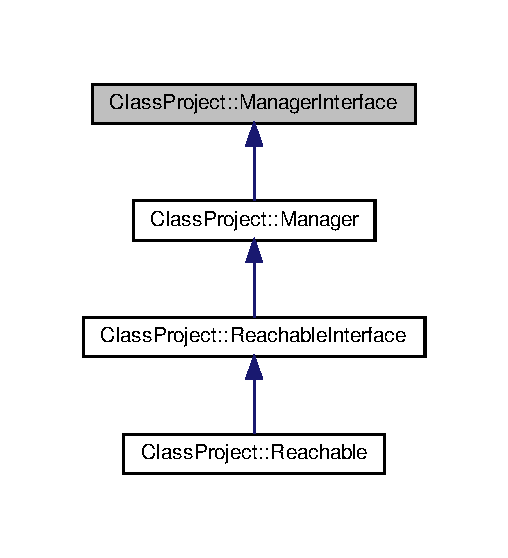
\includegraphics[width=244pt]{classClassProject_1_1ManagerInterface__inherit__graph}
\end{center}
\end{figure}
\subsection*{Public Member Functions}
\begin{DoxyCompactItemize}
\item 
\mbox{\Hypertarget{classClassProject_1_1ManagerInterface_ae2bf46167e81aa6c912bf8aff4202d17}\label{classClassProject_1_1ManagerInterface_ae2bf46167e81aa6c912bf8aff4202d17}} 
\hyperlink{classClassProject_1_1ManagerInterface_ae2bf46167e81aa6c912bf8aff4202d17}{Manager\+Interface} ()
\begin{DoxyCompactList}\small\item\em Constructor. \end{DoxyCompactList}\item 
virtual const B\+D\+D\+\_\+\+ID \& \hyperlink{classClassProject_1_1ManagerInterface_a104d0e8bcbd81eb501b66db6e24d1f63}{True} ()=0
\item 
virtual const B\+D\+D\+\_\+\+ID \& \hyperlink{classClassProject_1_1ManagerInterface_a98d18e1bc840fd664af015facfdcf690}{False} ()=0
\item 
virtual bool \hyperlink{classClassProject_1_1ManagerInterface_a0edd879f6ecae7bc5f84a2d55373d977}{is\+Constant} (const B\+D\+D\+\_\+\+ID f)=0
\item 
virtual bool \hyperlink{classClassProject_1_1ManagerInterface_a6eaaec7cbf8826198e490313ccb8f22a}{is\+Variable} (const B\+D\+D\+\_\+\+ID x)=0
\item 
virtual B\+D\+D\+\_\+\+ID \hyperlink{classClassProject_1_1ManagerInterface_ae2c645f859bcc7be3376d478f01eb045}{top\+Var} (const B\+D\+D\+\_\+\+ID f)=0
\item 
virtual B\+D\+D\+\_\+\+ID \hyperlink{classClassProject_1_1ManagerInterface_ab101acd3fbe6a5e29973d88f9862b8b4}{create\+Var} (const std\+::string \&label)=0
\item 
virtual B\+D\+D\+\_\+\+ID \hyperlink{classClassProject_1_1ManagerInterface_a6ea8f9482d86afb4128c52328d9ec11c}{ite} (const B\+D\+D\+\_\+\+ID i, const B\+D\+D\+\_\+\+ID t, const B\+D\+D\+\_\+\+ID e)=0
\item 
virtual B\+D\+D\+\_\+\+ID \hyperlink{classClassProject_1_1ManagerInterface_aab8496a0e551abdad99160e152199f4b}{co\+Factor\+True} (const B\+D\+D\+\_\+\+ID f, B\+D\+D\+\_\+\+ID x)=0
\item 
virtual B\+D\+D\+\_\+\+ID \hyperlink{classClassProject_1_1ManagerInterface_ad749ef1542c5b23bbbce628d6f666fe4}{co\+Factor\+False} (const B\+D\+D\+\_\+\+ID f, B\+D\+D\+\_\+\+ID x)=0
\item 
virtual B\+D\+D\+\_\+\+ID \hyperlink{classClassProject_1_1ManagerInterface_a4a1880d2245af9130646232551940949}{co\+Factor\+True} (const B\+D\+D\+\_\+\+ID f)=0
\item 
virtual B\+D\+D\+\_\+\+ID \hyperlink{classClassProject_1_1ManagerInterface_a308c99661ad02f407d6f2b0af6230e80}{co\+Factor\+False} (const B\+D\+D\+\_\+\+ID f)=0
\item 
virtual B\+D\+D\+\_\+\+ID \hyperlink{classClassProject_1_1ManagerInterface_af914326d34a1ed42710f7b11e5baf010}{and2} (const B\+D\+D\+\_\+\+ID a, const B\+D\+D\+\_\+\+ID b)=0
\item 
virtual B\+D\+D\+\_\+\+ID \hyperlink{classClassProject_1_1ManagerInterface_a8dbfde761b1e94d1f222b4d27f3c6fbc}{or2} (const B\+D\+D\+\_\+\+ID a, const B\+D\+D\+\_\+\+ID b)=0
\item 
virtual B\+D\+D\+\_\+\+ID \hyperlink{classClassProject_1_1ManagerInterface_a2b2c4948ef41ddb1036289cd07dac156}{xor2} (const B\+D\+D\+\_\+\+ID a, const B\+D\+D\+\_\+\+ID b)=0
\item 
virtual B\+D\+D\+\_\+\+ID \hyperlink{classClassProject_1_1ManagerInterface_a57d34af3121dcf5366d22ecf792f05a0}{neg} (const B\+D\+D\+\_\+\+ID a)=0
\item 
virtual B\+D\+D\+\_\+\+ID \hyperlink{classClassProject_1_1ManagerInterface_aaf6e357d680613e449d3ea958c9abba1}{nand2} (const B\+D\+D\+\_\+\+ID a, const B\+D\+D\+\_\+\+ID b)=0
\item 
virtual B\+D\+D\+\_\+\+ID \hyperlink{classClassProject_1_1ManagerInterface_a312d9865eae2d6355e17855cba78bc78}{nor2} (const B\+D\+D\+\_\+\+ID a, const B\+D\+D\+\_\+\+ID b)=0
\item 
virtual std\+::string \hyperlink{classClassProject_1_1ManagerInterface_afde45b2065361dfa6e61c1c7bc3fc1b4}{get\+Top\+Var\+Name} (const B\+D\+D\+\_\+\+ID \&root)=0
\item 
virtual void \hyperlink{classClassProject_1_1ManagerInterface_ab460e331ffdb85d4128574b3aae72c1e}{find\+Nodes} (const B\+D\+D\+\_\+\+ID \&root, std\+::set$<$ B\+D\+D\+\_\+\+ID $>$ \&nodes\+\_\+of\+\_\+root)=0
\item 
virtual void \hyperlink{classClassProject_1_1ManagerInterface_ab94feabca2125d334e542e502ae0186d}{find\+Vars} (const B\+D\+D\+\_\+\+ID \&root, std\+::set$<$ B\+D\+D\+\_\+\+ID $>$ \&vars\+\_\+of\+\_\+root)=0
\item 
virtual size\+\_\+t \hyperlink{classClassProject_1_1ManagerInterface_a85cac80444b26e5b80eb96b9f1231c0e}{unique\+Table\+Size} ()=0
\end{DoxyCompactItemize}


\subsection{Detailed Description}
Defines the implemented interface of the B\+DD package. 

\subsection{Member Function Documentation}
\mbox{\Hypertarget{classClassProject_1_1ManagerInterface_af914326d34a1ed42710f7b11e5baf010}\label{classClassProject_1_1ManagerInterface_af914326d34a1ed42710f7b11e5baf010}} 
\index{Class\+Project\+::\+Manager\+Interface@{Class\+Project\+::\+Manager\+Interface}!and2@{and2}}
\index{and2@{and2}!Class\+Project\+::\+Manager\+Interface@{Class\+Project\+::\+Manager\+Interface}}
\subsubsection{\texorpdfstring{and2()}{and2()}}
{\footnotesize\ttfamily virtual B\+D\+D\+\_\+\+ID Class\+Project\+::\+Manager\+Interface\+::and2 (\begin{DoxyParamCaption}\item[{const B\+D\+D\+\_\+\+ID}]{a,  }\item[{const B\+D\+D\+\_\+\+ID}]{b }\end{DoxyParamCaption})\hspace{0.3cm}{\ttfamily [pure virtual]}}

\begin{DoxyReturn}{Returns}
a B\+DD node that represents the correlating \char`\"{}and\char`\"{} function 
\end{DoxyReturn}


Implemented in \hyperlink{classClassProject_1_1Manager_a029fff4ef6650e4fd1f0ff37a69252de}{Class\+Project\+::\+Manager}.

\mbox{\Hypertarget{classClassProject_1_1ManagerInterface_ad749ef1542c5b23bbbce628d6f666fe4}\label{classClassProject_1_1ManagerInterface_ad749ef1542c5b23bbbce628d6f666fe4}} 
\index{Class\+Project\+::\+Manager\+Interface@{Class\+Project\+::\+Manager\+Interface}!co\+Factor\+False@{co\+Factor\+False}}
\index{co\+Factor\+False@{co\+Factor\+False}!Class\+Project\+::\+Manager\+Interface@{Class\+Project\+::\+Manager\+Interface}}
\subsubsection{\texorpdfstring{co\+Factor\+False()}{coFactorFalse()}\hspace{0.1cm}{\footnotesize\ttfamily [1/2]}}
{\footnotesize\ttfamily virtual B\+D\+D\+\_\+\+ID Class\+Project\+::\+Manager\+Interface\+::co\+Factor\+False (\begin{DoxyParamCaption}\item[{const B\+D\+D\+\_\+\+ID}]{f,  }\item[{B\+D\+D\+\_\+\+ID}]{x }\end{DoxyParamCaption})\hspace{0.3cm}{\ttfamily [pure virtual]}}

\begin{DoxyReturn}{Returns}
the negative cofactor of the function defined by f with respect to function x. 
\end{DoxyReturn}


Implemented in \hyperlink{classClassProject_1_1Manager_aea635ff0e0ec0cc8b43799f2d18de598}{Class\+Project\+::\+Manager}.

\mbox{\Hypertarget{classClassProject_1_1ManagerInterface_a308c99661ad02f407d6f2b0af6230e80}\label{classClassProject_1_1ManagerInterface_a308c99661ad02f407d6f2b0af6230e80}} 
\index{Class\+Project\+::\+Manager\+Interface@{Class\+Project\+::\+Manager\+Interface}!co\+Factor\+False@{co\+Factor\+False}}
\index{co\+Factor\+False@{co\+Factor\+False}!Class\+Project\+::\+Manager\+Interface@{Class\+Project\+::\+Manager\+Interface}}
\subsubsection{\texorpdfstring{co\+Factor\+False()}{coFactorFalse()}\hspace{0.1cm}{\footnotesize\ttfamily [2/2]}}
{\footnotesize\ttfamily virtual B\+D\+D\+\_\+\+ID Class\+Project\+::\+Manager\+Interface\+::co\+Factor\+False (\begin{DoxyParamCaption}\item[{const B\+D\+D\+\_\+\+ID}]{f }\end{DoxyParamCaption})\hspace{0.3cm}{\ttfamily [pure virtual]}}

\begin{DoxyReturn}{Returns}
the negative cofactor of the function defined by node f. 
\end{DoxyReturn}


Implemented in \hyperlink{classClassProject_1_1Manager_a3e3d13bac159441b8682338fe6a8bcb2}{Class\+Project\+::\+Manager}.

\mbox{\Hypertarget{classClassProject_1_1ManagerInterface_aab8496a0e551abdad99160e152199f4b}\label{classClassProject_1_1ManagerInterface_aab8496a0e551abdad99160e152199f4b}} 
\index{Class\+Project\+::\+Manager\+Interface@{Class\+Project\+::\+Manager\+Interface}!co\+Factor\+True@{co\+Factor\+True}}
\index{co\+Factor\+True@{co\+Factor\+True}!Class\+Project\+::\+Manager\+Interface@{Class\+Project\+::\+Manager\+Interface}}
\subsubsection{\texorpdfstring{co\+Factor\+True()}{coFactorTrue()}\hspace{0.1cm}{\footnotesize\ttfamily [1/2]}}
{\footnotesize\ttfamily virtual B\+D\+D\+\_\+\+ID Class\+Project\+::\+Manager\+Interface\+::co\+Factor\+True (\begin{DoxyParamCaption}\item[{const B\+D\+D\+\_\+\+ID}]{f,  }\item[{B\+D\+D\+\_\+\+ID}]{x }\end{DoxyParamCaption})\hspace{0.3cm}{\ttfamily [pure virtual]}}

\begin{DoxyReturn}{Returns}
the positive cofactor of the function defined by f with respect to function x. 
\end{DoxyReturn}


Implemented in \hyperlink{classClassProject_1_1Manager_aa2bfdbb0fae8e09b2b766336cdf7ce94}{Class\+Project\+::\+Manager}.

\mbox{\Hypertarget{classClassProject_1_1ManagerInterface_a4a1880d2245af9130646232551940949}\label{classClassProject_1_1ManagerInterface_a4a1880d2245af9130646232551940949}} 
\index{Class\+Project\+::\+Manager\+Interface@{Class\+Project\+::\+Manager\+Interface}!co\+Factor\+True@{co\+Factor\+True}}
\index{co\+Factor\+True@{co\+Factor\+True}!Class\+Project\+::\+Manager\+Interface@{Class\+Project\+::\+Manager\+Interface}}
\subsubsection{\texorpdfstring{co\+Factor\+True()}{coFactorTrue()}\hspace{0.1cm}{\footnotesize\ttfamily [2/2]}}
{\footnotesize\ttfamily virtual B\+D\+D\+\_\+\+ID Class\+Project\+::\+Manager\+Interface\+::co\+Factor\+True (\begin{DoxyParamCaption}\item[{const B\+D\+D\+\_\+\+ID}]{f }\end{DoxyParamCaption})\hspace{0.3cm}{\ttfamily [pure virtual]}}

\begin{DoxyReturn}{Returns}
the positive cofactor of the function defined by node f. 
\end{DoxyReturn}


Implemented in \hyperlink{classClassProject_1_1Manager_ab2b73e9169e978c45a4ebf9aa3bddef8}{Class\+Project\+::\+Manager}.

\mbox{\Hypertarget{classClassProject_1_1ManagerInterface_ab101acd3fbe6a5e29973d88f9862b8b4}\label{classClassProject_1_1ManagerInterface_ab101acd3fbe6a5e29973d88f9862b8b4}} 
\index{Class\+Project\+::\+Manager\+Interface@{Class\+Project\+::\+Manager\+Interface}!create\+Var@{create\+Var}}
\index{create\+Var@{create\+Var}!Class\+Project\+::\+Manager\+Interface@{Class\+Project\+::\+Manager\+Interface}}
\subsubsection{\texorpdfstring{create\+Var()}{createVar()}}
{\footnotesize\ttfamily virtual B\+D\+D\+\_\+\+ID Class\+Project\+::\+Manager\+Interface\+::create\+Var (\begin{DoxyParamCaption}\item[{const std\+::string \&}]{label }\end{DoxyParamCaption})\hspace{0.3cm}{\ttfamily [pure virtual]}}

Creates a new variable for the B\+DD. 

Implemented in \hyperlink{classClassProject_1_1Manager_a9fb480d8af44c75ee2b35b85f7038e68}{Class\+Project\+::\+Manager}.

\mbox{\Hypertarget{classClassProject_1_1ManagerInterface_a98d18e1bc840fd664af015facfdcf690}\label{classClassProject_1_1ManagerInterface_a98d18e1bc840fd664af015facfdcf690}} 
\index{Class\+Project\+::\+Manager\+Interface@{Class\+Project\+::\+Manager\+Interface}!False@{False}}
\index{False@{False}!Class\+Project\+::\+Manager\+Interface@{Class\+Project\+::\+Manager\+Interface}}
\subsubsection{\texorpdfstring{False()}{False()}}
{\footnotesize\ttfamily virtual const B\+D\+D\+\_\+\+ID\& Class\+Project\+::\+Manager\+Interface\+::\+False (\begin{DoxyParamCaption}{ }\end{DoxyParamCaption})\hspace{0.3cm}{\ttfamily [pure virtual]}}

\begin{DoxyReturn}{Returns}
the ID of the node representing False. 
\end{DoxyReturn}


Implemented in \hyperlink{classClassProject_1_1Manager_ae9bae01509e6063313024cd85a8eb569}{Class\+Project\+::\+Manager}.

\mbox{\Hypertarget{classClassProject_1_1ManagerInterface_ab460e331ffdb85d4128574b3aae72c1e}\label{classClassProject_1_1ManagerInterface_ab460e331ffdb85d4128574b3aae72c1e}} 
\index{Class\+Project\+::\+Manager\+Interface@{Class\+Project\+::\+Manager\+Interface}!find\+Nodes@{find\+Nodes}}
\index{find\+Nodes@{find\+Nodes}!Class\+Project\+::\+Manager\+Interface@{Class\+Project\+::\+Manager\+Interface}}
\subsubsection{\texorpdfstring{find\+Nodes()}{findNodes()}}
{\footnotesize\ttfamily virtual void Class\+Project\+::\+Manager\+Interface\+::find\+Nodes (\begin{DoxyParamCaption}\item[{const B\+D\+D\+\_\+\+ID \&}]{root,  }\item[{std\+::set$<$ B\+D\+D\+\_\+\+ID $>$ \&}]{nodes\+\_\+of\+\_\+root }\end{DoxyParamCaption})\hspace{0.3cm}{\ttfamily [pure virtual]}}

\begin{DoxyReturn}{Returns}
the set of B\+DD nodes which are reachable from the B\+DD node root (including itself). 
\end{DoxyReturn}


Implemented in \hyperlink{classClassProject_1_1Manager_a2aefec8f025f8d7417eff8493bcd7f04}{Class\+Project\+::\+Manager}.

\mbox{\Hypertarget{classClassProject_1_1ManagerInterface_ab94feabca2125d334e542e502ae0186d}\label{classClassProject_1_1ManagerInterface_ab94feabca2125d334e542e502ae0186d}} 
\index{Class\+Project\+::\+Manager\+Interface@{Class\+Project\+::\+Manager\+Interface}!find\+Vars@{find\+Vars}}
\index{find\+Vars@{find\+Vars}!Class\+Project\+::\+Manager\+Interface@{Class\+Project\+::\+Manager\+Interface}}
\subsubsection{\texorpdfstring{find\+Vars()}{findVars()}}
{\footnotesize\ttfamily virtual void Class\+Project\+::\+Manager\+Interface\+::find\+Vars (\begin{DoxyParamCaption}\item[{const B\+D\+D\+\_\+\+ID \&}]{root,  }\item[{std\+::set$<$ B\+D\+D\+\_\+\+ID $>$ \&}]{vars\+\_\+of\+\_\+root }\end{DoxyParamCaption})\hspace{0.3cm}{\ttfamily [pure virtual]}}

\begin{DoxyReturn}{Returns}
the set of variables which are either top variable of the B\+DD node root or the reachable nodes from root. 
\end{DoxyReturn}


Implemented in \hyperlink{classClassProject_1_1Manager_abf869470f4d1baffca8a140d3196c2ad}{Class\+Project\+::\+Manager}.

\mbox{\Hypertarget{classClassProject_1_1ManagerInterface_afde45b2065361dfa6e61c1c7bc3fc1b4}\label{classClassProject_1_1ManagerInterface_afde45b2065361dfa6e61c1c7bc3fc1b4}} 
\index{Class\+Project\+::\+Manager\+Interface@{Class\+Project\+::\+Manager\+Interface}!get\+Top\+Var\+Name@{get\+Top\+Var\+Name}}
\index{get\+Top\+Var\+Name@{get\+Top\+Var\+Name}!Class\+Project\+::\+Manager\+Interface@{Class\+Project\+::\+Manager\+Interface}}
\subsubsection{\texorpdfstring{get\+Top\+Var\+Name()}{getTopVarName()}}
{\footnotesize\ttfamily virtual std\+::string Class\+Project\+::\+Manager\+Interface\+::get\+Top\+Var\+Name (\begin{DoxyParamCaption}\item[{const B\+D\+D\+\_\+\+ID \&}]{root }\end{DoxyParamCaption})\hspace{0.3cm}{\ttfamily [pure virtual]}}

\begin{DoxyReturn}{Returns}
the Name of top variable of the B\+DD node root 
\end{DoxyReturn}


Implemented in \hyperlink{classClassProject_1_1Manager_a72e49c79e186bfce423eb554cca28ff2}{Class\+Project\+::\+Manager}.

\mbox{\Hypertarget{classClassProject_1_1ManagerInterface_a0edd879f6ecae7bc5f84a2d55373d977}\label{classClassProject_1_1ManagerInterface_a0edd879f6ecae7bc5f84a2d55373d977}} 
\index{Class\+Project\+::\+Manager\+Interface@{Class\+Project\+::\+Manager\+Interface}!is\+Constant@{is\+Constant}}
\index{is\+Constant@{is\+Constant}!Class\+Project\+::\+Manager\+Interface@{Class\+Project\+::\+Manager\+Interface}}
\subsubsection{\texorpdfstring{is\+Constant()}{isConstant()}}
{\footnotesize\ttfamily virtual bool Class\+Project\+::\+Manager\+Interface\+::is\+Constant (\begin{DoxyParamCaption}\item[{const B\+D\+D\+\_\+\+ID}]{f }\end{DoxyParamCaption})\hspace{0.3cm}{\ttfamily [pure virtual]}}

\begin{DoxyReturn}{Returns}
true if x is a leaf node. 
\end{DoxyReturn}


Implemented in \hyperlink{classClassProject_1_1Manager_a98fe06b67d8114f1404a7b19dddc935b}{Class\+Project\+::\+Manager}.

\mbox{\Hypertarget{classClassProject_1_1ManagerInterface_a6eaaec7cbf8826198e490313ccb8f22a}\label{classClassProject_1_1ManagerInterface_a6eaaec7cbf8826198e490313ccb8f22a}} 
\index{Class\+Project\+::\+Manager\+Interface@{Class\+Project\+::\+Manager\+Interface}!is\+Variable@{is\+Variable}}
\index{is\+Variable@{is\+Variable}!Class\+Project\+::\+Manager\+Interface@{Class\+Project\+::\+Manager\+Interface}}
\subsubsection{\texorpdfstring{is\+Variable()}{isVariable()}}
{\footnotesize\ttfamily virtual bool Class\+Project\+::\+Manager\+Interface\+::is\+Variable (\begin{DoxyParamCaption}\item[{const B\+D\+D\+\_\+\+ID}]{x }\end{DoxyParamCaption})\hspace{0.3cm}{\ttfamily [pure virtual]}}

\begin{DoxyReturn}{Returns}
true if x is a variable. 
\end{DoxyReturn}


Implemented in \hyperlink{classClassProject_1_1Manager_af026f76f68823bb9083f161b5db9e58b}{Class\+Project\+::\+Manager}.

\mbox{\Hypertarget{classClassProject_1_1ManagerInterface_a6ea8f9482d86afb4128c52328d9ec11c}\label{classClassProject_1_1ManagerInterface_a6ea8f9482d86afb4128c52328d9ec11c}} 
\index{Class\+Project\+::\+Manager\+Interface@{Class\+Project\+::\+Manager\+Interface}!ite@{ite}}
\index{ite@{ite}!Class\+Project\+::\+Manager\+Interface@{Class\+Project\+::\+Manager\+Interface}}
\subsubsection{\texorpdfstring{ite()}{ite()}}
{\footnotesize\ttfamily virtual B\+D\+D\+\_\+\+ID Class\+Project\+::\+Manager\+Interface\+::ite (\begin{DoxyParamCaption}\item[{const B\+D\+D\+\_\+\+ID}]{i,  }\item[{const B\+D\+D\+\_\+\+ID}]{t,  }\item[{const B\+D\+D\+\_\+\+ID}]{e }\end{DoxyParamCaption})\hspace{0.3cm}{\ttfamily [pure virtual]}}

Implements the if-\/then-\/else algorithm. \begin{DoxyReturn}{Returns}
the new node that represents the I\+TE. 
\end{DoxyReturn}


Implemented in \hyperlink{classClassProject_1_1Manager_ab6b8135aadc0a5b91b5c651c4046da05}{Class\+Project\+::\+Manager}.

\mbox{\Hypertarget{classClassProject_1_1ManagerInterface_aaf6e357d680613e449d3ea958c9abba1}\label{classClassProject_1_1ManagerInterface_aaf6e357d680613e449d3ea958c9abba1}} 
\index{Class\+Project\+::\+Manager\+Interface@{Class\+Project\+::\+Manager\+Interface}!nand2@{nand2}}
\index{nand2@{nand2}!Class\+Project\+::\+Manager\+Interface@{Class\+Project\+::\+Manager\+Interface}}
\subsubsection{\texorpdfstring{nand2()}{nand2()}}
{\footnotesize\ttfamily virtual B\+D\+D\+\_\+\+ID Class\+Project\+::\+Manager\+Interface\+::nand2 (\begin{DoxyParamCaption}\item[{const B\+D\+D\+\_\+\+ID}]{a,  }\item[{const B\+D\+D\+\_\+\+ID}]{b }\end{DoxyParamCaption})\hspace{0.3cm}{\ttfamily [pure virtual]}}

\begin{DoxyReturn}{Returns}
a B\+DD node that represents the correlating \char`\"{}nand\char`\"{} function 
\end{DoxyReturn}


Implemented in \hyperlink{classClassProject_1_1Manager_abde082c99a3588ad7e25b620e901e6e0}{Class\+Project\+::\+Manager}.

\mbox{\Hypertarget{classClassProject_1_1ManagerInterface_a57d34af3121dcf5366d22ecf792f05a0}\label{classClassProject_1_1ManagerInterface_a57d34af3121dcf5366d22ecf792f05a0}} 
\index{Class\+Project\+::\+Manager\+Interface@{Class\+Project\+::\+Manager\+Interface}!neg@{neg}}
\index{neg@{neg}!Class\+Project\+::\+Manager\+Interface@{Class\+Project\+::\+Manager\+Interface}}
\subsubsection{\texorpdfstring{neg()}{neg()}}
{\footnotesize\ttfamily virtual B\+D\+D\+\_\+\+ID Class\+Project\+::\+Manager\+Interface\+::neg (\begin{DoxyParamCaption}\item[{const B\+D\+D\+\_\+\+ID}]{a }\end{DoxyParamCaption})\hspace{0.3cm}{\ttfamily [pure virtual]}}

\begin{DoxyReturn}{Returns}
a B\+DD node that represents the correlating \char`\"{}neg\char`\"{} function 
\end{DoxyReturn}


Implemented in \hyperlink{classClassProject_1_1Manager_ab53a25ffc83724427725347ed3f9e6ce}{Class\+Project\+::\+Manager}.

\mbox{\Hypertarget{classClassProject_1_1ManagerInterface_a312d9865eae2d6355e17855cba78bc78}\label{classClassProject_1_1ManagerInterface_a312d9865eae2d6355e17855cba78bc78}} 
\index{Class\+Project\+::\+Manager\+Interface@{Class\+Project\+::\+Manager\+Interface}!nor2@{nor2}}
\index{nor2@{nor2}!Class\+Project\+::\+Manager\+Interface@{Class\+Project\+::\+Manager\+Interface}}
\subsubsection{\texorpdfstring{nor2()}{nor2()}}
{\footnotesize\ttfamily virtual B\+D\+D\+\_\+\+ID Class\+Project\+::\+Manager\+Interface\+::nor2 (\begin{DoxyParamCaption}\item[{const B\+D\+D\+\_\+\+ID}]{a,  }\item[{const B\+D\+D\+\_\+\+ID}]{b }\end{DoxyParamCaption})\hspace{0.3cm}{\ttfamily [pure virtual]}}

\begin{DoxyReturn}{Returns}
a B\+DD node that represents the correlating \char`\"{}nor\char`\"{} function 
\end{DoxyReturn}


Implemented in \hyperlink{classClassProject_1_1Manager_a1cbba8dc08a8c1bbabce0b98a8fde3be}{Class\+Project\+::\+Manager}.

\mbox{\Hypertarget{classClassProject_1_1ManagerInterface_a8dbfde761b1e94d1f222b4d27f3c6fbc}\label{classClassProject_1_1ManagerInterface_a8dbfde761b1e94d1f222b4d27f3c6fbc}} 
\index{Class\+Project\+::\+Manager\+Interface@{Class\+Project\+::\+Manager\+Interface}!or2@{or2}}
\index{or2@{or2}!Class\+Project\+::\+Manager\+Interface@{Class\+Project\+::\+Manager\+Interface}}
\subsubsection{\texorpdfstring{or2()}{or2()}}
{\footnotesize\ttfamily virtual B\+D\+D\+\_\+\+ID Class\+Project\+::\+Manager\+Interface\+::or2 (\begin{DoxyParamCaption}\item[{const B\+D\+D\+\_\+\+ID}]{a,  }\item[{const B\+D\+D\+\_\+\+ID}]{b }\end{DoxyParamCaption})\hspace{0.3cm}{\ttfamily [pure virtual]}}

\begin{DoxyReturn}{Returns}
a B\+DD node that represents the correlating \char`\"{}or\char`\"{} function 
\end{DoxyReturn}


Implemented in \hyperlink{classClassProject_1_1Manager_a0f415b7af83a3efb6f7020650e68f1c3}{Class\+Project\+::\+Manager}.

\mbox{\Hypertarget{classClassProject_1_1ManagerInterface_ae2c645f859bcc7be3376d478f01eb045}\label{classClassProject_1_1ManagerInterface_ae2c645f859bcc7be3376d478f01eb045}} 
\index{Class\+Project\+::\+Manager\+Interface@{Class\+Project\+::\+Manager\+Interface}!top\+Var@{top\+Var}}
\index{top\+Var@{top\+Var}!Class\+Project\+::\+Manager\+Interface@{Class\+Project\+::\+Manager\+Interface}}
\subsubsection{\texorpdfstring{top\+Var()}{topVar()}}
{\footnotesize\ttfamily virtual B\+D\+D\+\_\+\+ID Class\+Project\+::\+Manager\+Interface\+::top\+Var (\begin{DoxyParamCaption}\item[{const B\+D\+D\+\_\+\+ID}]{f }\end{DoxyParamCaption})\hspace{0.3cm}{\ttfamily [pure virtual]}}

\begin{DoxyReturn}{Returns}
the ID of top variable of the B\+DD node f 
\end{DoxyReturn}


Implemented in \hyperlink{classClassProject_1_1Manager_a8ddf48759e4e3a5c9e92b07470372b7e}{Class\+Project\+::\+Manager}.

\mbox{\Hypertarget{classClassProject_1_1ManagerInterface_a104d0e8bcbd81eb501b66db6e24d1f63}\label{classClassProject_1_1ManagerInterface_a104d0e8bcbd81eb501b66db6e24d1f63}} 
\index{Class\+Project\+::\+Manager\+Interface@{Class\+Project\+::\+Manager\+Interface}!True@{True}}
\index{True@{True}!Class\+Project\+::\+Manager\+Interface@{Class\+Project\+::\+Manager\+Interface}}
\subsubsection{\texorpdfstring{True()}{True()}}
{\footnotesize\ttfamily virtual const B\+D\+D\+\_\+\+ID\& Class\+Project\+::\+Manager\+Interface\+::\+True (\begin{DoxyParamCaption}{ }\end{DoxyParamCaption})\hspace{0.3cm}{\ttfamily [pure virtual]}}

\begin{DoxyReturn}{Returns}
the ID of the node representing True. 
\end{DoxyReturn}


Implemented in \hyperlink{classClassProject_1_1Manager_a0c15aff167a7019502b66100c4ec0a33}{Class\+Project\+::\+Manager}.

\mbox{\Hypertarget{classClassProject_1_1ManagerInterface_a85cac80444b26e5b80eb96b9f1231c0e}\label{classClassProject_1_1ManagerInterface_a85cac80444b26e5b80eb96b9f1231c0e}} 
\index{Class\+Project\+::\+Manager\+Interface@{Class\+Project\+::\+Manager\+Interface}!unique\+Table\+Size@{unique\+Table\+Size}}
\index{unique\+Table\+Size@{unique\+Table\+Size}!Class\+Project\+::\+Manager\+Interface@{Class\+Project\+::\+Manager\+Interface}}
\subsubsection{\texorpdfstring{unique\+Table\+Size()}{uniqueTableSize()}}
{\footnotesize\ttfamily virtual size\+\_\+t Class\+Project\+::\+Manager\+Interface\+::unique\+Table\+Size (\begin{DoxyParamCaption}{ }\end{DoxyParamCaption})\hspace{0.3cm}{\ttfamily [pure virtual]}}

\begin{DoxyReturn}{Returns}
the number of the nodes currently exist in the unique table of the \hyperlink{classClassProject_1_1Manager}{Manager} class. 
\end{DoxyReturn}


Implemented in \hyperlink{classClassProject_1_1Manager_a82b10a42ec726d42ea4d2e8bc72a3db9}{Class\+Project\+::\+Manager}.

\mbox{\Hypertarget{classClassProject_1_1ManagerInterface_a2b2c4948ef41ddb1036289cd07dac156}\label{classClassProject_1_1ManagerInterface_a2b2c4948ef41ddb1036289cd07dac156}} 
\index{Class\+Project\+::\+Manager\+Interface@{Class\+Project\+::\+Manager\+Interface}!xor2@{xor2}}
\index{xor2@{xor2}!Class\+Project\+::\+Manager\+Interface@{Class\+Project\+::\+Manager\+Interface}}
\subsubsection{\texorpdfstring{xor2()}{xor2()}}
{\footnotesize\ttfamily virtual B\+D\+D\+\_\+\+ID Class\+Project\+::\+Manager\+Interface\+::xor2 (\begin{DoxyParamCaption}\item[{const B\+D\+D\+\_\+\+ID}]{a,  }\item[{const B\+D\+D\+\_\+\+ID}]{b }\end{DoxyParamCaption})\hspace{0.3cm}{\ttfamily [pure virtual]}}

\begin{DoxyReturn}{Returns}
a B\+DD node that represents the correlating \char`\"{}xor\char`\"{} function 
\end{DoxyReturn}


Implemented in \hyperlink{classClassProject_1_1Manager_a2582e9a9474189a2710c551548c20c19}{Class\+Project\+::\+Manager}.


\hypertarget{classClassProject_1_1Reachable}{}\section{Class\+Project\+:\+:Reachable Class Reference}
\label{classClassProject_1_1Reachable}\index{Class\+Project\+::\+Reachable@{Class\+Project\+::\+Reachable}}


Implements the interface of the reachability extension.  




{\ttfamily \#include $<$Reachable.\+h$>$}



Inheritance diagram for Class\+Project\+:\+:Reachable\+:
\nopagebreak
\begin{figure}[H]
\begin{center}
\leavevmode
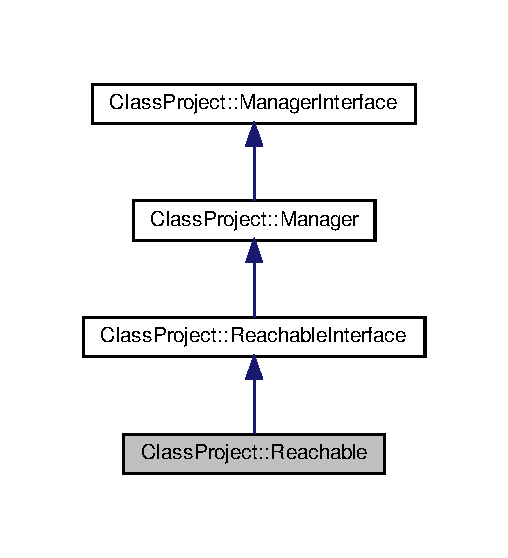
\includegraphics[width=244pt]{classClassProject_1_1Reachable__inherit__graph}
\end{center}
\end{figure}


Collaboration diagram for Class\+Project\+:\+:Reachable\+:
\nopagebreak
\begin{figure}[H]
\begin{center}
\leavevmode
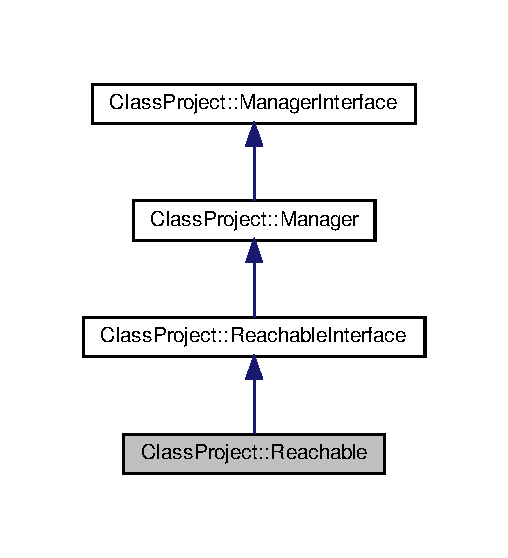
\includegraphics[width=244pt]{classClassProject_1_1Reachable__coll__graph}
\end{center}
\end{figure}
\subsection*{Public Member Functions}
\begin{DoxyCompactItemize}
\item 
\hyperlink{classClassProject_1_1Reachable_ab5198f10bf77a813a7547bb5cbf72fc9}{Reachable} (unsigned int state\+Size)
\begin{DoxyCompactList}\small\item\em Constructor. \end{DoxyCompactList}\item 
\hyperlink{classClassProject_1_1Reachable_a1f39c60e57237bf1af65657f41a58c2f}{$\sim$\+Reachable} () override=default
\item 
\mbox{\Hypertarget{classClassProject_1_1Reachable_aef184d12beb7264228104f04d4aef63e}\label{classClassProject_1_1Reachable_aef184d12beb7264228104f04d4aef63e}} 
void {\bfseries check\+\_\+size\+\_\+array} (const std\+::vector$<$ B\+D\+D\+\_\+\+ID $>$ \&array)
\item 
\mbox{\Hypertarget{classClassProject_1_1Reachable_ab1112c527e5a944129b61d9566ca6186}\label{classClassProject_1_1Reachable_ab1112c527e5a944129b61d9566ca6186}} 
void {\bfseries check\+\_\+size\+\_\+array} (const std\+::vector$<$ bool $>$ \&array)
\item 
B\+D\+D\+\_\+\+ID \hyperlink{classClassProject_1_1Reachable_a7f97f9868c825b64f333c4bc8eb7632b}{xnor2} (B\+D\+D\+\_\+\+ID a, B\+D\+D\+\_\+\+ID b) override
\item 
const std\+::vector$<$ B\+D\+D\+\_\+\+ID $>$ \& \hyperlink{classClassProject_1_1Reachable_a46b6aab8ea4dac374af4e2e97b5321dd}{get\+States} () const override
\item 
void \hyperlink{classClassProject_1_1Reachable_a53fdcc94c37cd7f0e27881678189b5c5}{set\+Delta} (const std\+::vector$<$ B\+D\+D\+\_\+\+ID $>$ \&transition\+Functions) override
\item 
const std\+::vector$<$ B\+D\+D\+\_\+\+ID $>$ \& \hyperlink{classClassProject_1_1Reachable_a52a7381b5237c686f47496b8c63ac37f}{get\+Delta} () const
\item 
void \hyperlink{classClassProject_1_1Reachable_ab3ddc3f569e280c3902a40ab8202f8c3}{set\+Init\+State} (const std\+::vector$<$ bool $>$ \&state\+Vector) override
\item 
const std\+::vector$<$ bool $>$ \& \hyperlink{classClassProject_1_1Reachable_a713e76e60c325f459c4561517fd832b6}{get\+Init\+State} () const
\item 
B\+D\+D\+\_\+\+ID \hyperlink{classClassProject_1_1Reachable_ab382d204af0fe91f027026b6dad6142f}{compute\+\_\+reachable\+\_\+states} () override
\item 
bool \hyperlink{classClassProject_1_1Reachable_a19a40b477fc119690e0a9f1f7ffc4843}{is\+\_\+reachable} (const std\+::vector$<$ bool $>$ \&state\+Vector) override
\end{DoxyCompactItemize}


\subsection{Detailed Description}
Implements the interface of the reachability extension. 

\subsection{Constructor \& Destructor Documentation}
\mbox{\Hypertarget{classClassProject_1_1Reachable_ab5198f10bf77a813a7547bb5cbf72fc9}\label{classClassProject_1_1Reachable_ab5198f10bf77a813a7547bb5cbf72fc9}} 
\index{Class\+Project\+::\+Reachable@{Class\+Project\+::\+Reachable}!Reachable@{Reachable}}
\index{Reachable@{Reachable}!Class\+Project\+::\+Reachable@{Class\+Project\+::\+Reachable}}
\subsubsection{\texorpdfstring{Reachable()}{Reachable()}}
{\footnotesize\ttfamily Class\+Project\+::\+Reachable\+::\+Reachable (\begin{DoxyParamCaption}\item[{unsigned int}]{state\+Size }\end{DoxyParamCaption})\hspace{0.3cm}{\ttfamily [explicit]}}



Constructor. 

This constructor creates the data structures required for the reachability analysis. It also initializes them according to number of state bits. \mbox{\Hypertarget{classClassProject_1_1Reachable_a1f39c60e57237bf1af65657f41a58c2f}\label{classClassProject_1_1Reachable_a1f39c60e57237bf1af65657f41a58c2f}} 
\index{Class\+Project\+::\+Reachable@{Class\+Project\+::\+Reachable}!````~Reachable@{$\sim$\+Reachable}}
\index{````~Reachable@{$\sim$\+Reachable}!Class\+Project\+::\+Reachable@{Class\+Project\+::\+Reachable}}
\subsubsection{\texorpdfstring{$\sim$\+Reachable()}{~Reachable()}}
{\footnotesize\ttfamily Class\+Project\+::\+Reachable\+::$\sim$\+Reachable (\begin{DoxyParamCaption}{ }\end{DoxyParamCaption})\hspace{0.3cm}{\ttfamily [override]}, {\ttfamily [default]}}

Destructor 

\subsection{Member Function Documentation}
\mbox{\Hypertarget{classClassProject_1_1Reachable_ab382d204af0fe91f027026b6dad6142f}\label{classClassProject_1_1Reachable_ab382d204af0fe91f027026b6dad6142f}} 
\index{Class\+Project\+::\+Reachable@{Class\+Project\+::\+Reachable}!compute\+\_\+reachable\+\_\+states@{compute\+\_\+reachable\+\_\+states}}
\index{compute\+\_\+reachable\+\_\+states@{compute\+\_\+reachable\+\_\+states}!Class\+Project\+::\+Reachable@{Class\+Project\+::\+Reachable}}
\subsubsection{\texorpdfstring{compute\+\_\+reachable\+\_\+states()}{compute\_reachable\_states()}}
{\footnotesize\ttfamily B\+D\+D\+\_\+\+ID Class\+Project\+::\+Reachable\+::compute\+\_\+reachable\+\_\+states (\begin{DoxyParamCaption}{ }\end{DoxyParamCaption})\hspace{0.3cm}{\ttfamily [override]}, {\ttfamily [virtual]}}

Computes the symbolic representation of the reachable states. Before this method is called it is important to set the transition function and the initial state. \begin{DoxyReturn}{Returns}
B\+D\+D\+\_\+\+ID of the reachable state space 
\end{DoxyReturn}


Implements \hyperlink{classClassProject_1_1ReachableInterface_a84a2fe53f724c184266fc22f17204499}{Class\+Project\+::\+Reachable\+Interface}.

\mbox{\Hypertarget{classClassProject_1_1Reachable_a52a7381b5237c686f47496b8c63ac37f}\label{classClassProject_1_1Reachable_a52a7381b5237c686f47496b8c63ac37f}} 
\index{Class\+Project\+::\+Reachable@{Class\+Project\+::\+Reachable}!get\+Delta@{get\+Delta}}
\index{get\+Delta@{get\+Delta}!Class\+Project\+::\+Reachable@{Class\+Project\+::\+Reachable}}
\subsubsection{\texorpdfstring{get\+Delta()}{getDelta()}}
{\footnotesize\ttfamily const std\+::vector$<$ B\+D\+D\+\_\+\+ID $>$ \& Class\+Project\+::\+Reachable\+::get\+Delta (\begin{DoxyParamCaption}{ }\end{DoxyParamCaption}) const}

Each state variable has a transition function. The transition function specifies the value of the state after the transition. The transition function are composed of only state variables. For example\+: s0\textquotesingle{} = s0 X\+OR s1 The next state is defined as X\+OR of the current values of the state bit s0 and s1 \begin{DoxyReturn}{Returns}
vector with the B\+D\+D\+\_\+\+ID or the transition functions 
\end{DoxyReturn}
\mbox{\Hypertarget{classClassProject_1_1Reachable_a713e76e60c325f459c4561517fd832b6}\label{classClassProject_1_1Reachable_a713e76e60c325f459c4561517fd832b6}} 
\index{Class\+Project\+::\+Reachable@{Class\+Project\+::\+Reachable}!get\+Init\+State@{get\+Init\+State}}
\index{get\+Init\+State@{get\+Init\+State}!Class\+Project\+::\+Reachable@{Class\+Project\+::\+Reachable}}
\subsubsection{\texorpdfstring{get\+Init\+State()}{getInitState()}}
{\footnotesize\ttfamily const std\+::vector$<$ bool $>$ \& Class\+Project\+::\+Reachable\+::get\+Init\+State (\begin{DoxyParamCaption}{ }\end{DoxyParamCaption}) const}

Each state machine has an initial state. The initial state is provided as a vector. The vector has to have an entry for each state bit. If the entry is \char`\"{}true\char`\"{} the state bit is high, otherwise negated. E.\+g. initial state not(s0) and not(s1) is transformed into \{false,false\}. 
\begin{DoxyParams}{Parameters}
{\em state\+Vector} & provide the assignment for each state bit \\
\hline
\end{DoxyParams}
\mbox{\Hypertarget{classClassProject_1_1Reachable_a46b6aab8ea4dac374af4e2e97b5321dd}\label{classClassProject_1_1Reachable_a46b6aab8ea4dac374af4e2e97b5321dd}} 
\index{Class\+Project\+::\+Reachable@{Class\+Project\+::\+Reachable}!get\+States@{get\+States}}
\index{get\+States@{get\+States}!Class\+Project\+::\+Reachable@{Class\+Project\+::\+Reachable}}
\subsubsection{\texorpdfstring{get\+States()}{getStates()}}
{\footnotesize\ttfamily const std\+::vector$<$ B\+D\+D\+\_\+\+ID $>$ \& Class\+Project\+::\+Reachable\+::get\+States (\begin{DoxyParamCaption}{ }\end{DoxyParamCaption}) const\hspace{0.3cm}{\ttfamily [override]}, {\ttfamily [virtual]}}

States are generated and stored in a vector. These lsb (e.\+g. \char`\"{}s0\char`\"{}) is stored at location 0. The msb(e.\+g. \char`\"{}s3\char`\"{}) is stored at location size-\/1. \begin{DoxyReturn}{Returns}
vector with the B\+D\+D\+\_\+\+ID of each state bit 
\end{DoxyReturn}


Implements \hyperlink{classClassProject_1_1ReachableInterface_a8546499fbc6d0da61b6b21f8db8e4621}{Class\+Project\+::\+Reachable\+Interface}.

\mbox{\Hypertarget{classClassProject_1_1Reachable_a19a40b477fc119690e0a9f1f7ffc4843}\label{classClassProject_1_1Reachable_a19a40b477fc119690e0a9f1f7ffc4843}} 
\index{Class\+Project\+::\+Reachable@{Class\+Project\+::\+Reachable}!is\+\_\+reachable@{is\+\_\+reachable}}
\index{is\+\_\+reachable@{is\+\_\+reachable}!Class\+Project\+::\+Reachable@{Class\+Project\+::\+Reachable}}
\subsubsection{\texorpdfstring{is\+\_\+reachable()}{is\_reachable()}}
{\footnotesize\ttfamily bool Class\+Project\+::\+Reachable\+::is\+\_\+reachable (\begin{DoxyParamCaption}\item[{const std\+::vector$<$ bool $>$ \&}]{state\+Vector }\end{DoxyParamCaption})\hspace{0.3cm}{\ttfamily [override]}, {\ttfamily [virtual]}}

This method decides whether a specific state is in the reachable state space or not. The input is provided as a vector of states. The value is true if the state bit is high in this state, false otherwise. 
\begin{DoxyParams}{Parameters}
{\em state\+Vector} & \\
\hline
\end{DoxyParams}
\begin{DoxyReturn}{Returns}
Boolean indicating if the state is reachable 
\end{DoxyReturn}


Implements \hyperlink{classClassProject_1_1ReachableInterface_aa3011f06562431832cf563b77fb36c13}{Class\+Project\+::\+Reachable\+Interface}.

\mbox{\Hypertarget{classClassProject_1_1Reachable_a53fdcc94c37cd7f0e27881678189b5c5}\label{classClassProject_1_1Reachable_a53fdcc94c37cd7f0e27881678189b5c5}} 
\index{Class\+Project\+::\+Reachable@{Class\+Project\+::\+Reachable}!set\+Delta@{set\+Delta}}
\index{set\+Delta@{set\+Delta}!Class\+Project\+::\+Reachable@{Class\+Project\+::\+Reachable}}
\subsubsection{\texorpdfstring{set\+Delta()}{setDelta()}}
{\footnotesize\ttfamily void Class\+Project\+::\+Reachable\+::set\+Delta (\begin{DoxyParamCaption}\item[{const std\+::vector$<$ B\+D\+D\+\_\+\+ID $>$ \&}]{transition\+Functions }\end{DoxyParamCaption})\hspace{0.3cm}{\ttfamily [override]}, {\ttfamily [virtual]}}

Each state variable has a transition function. The transition function specifies the value of the state after the transition. The transition function are composed of only state variables. For example\+: s0\textquotesingle{} = s0 X\+OR s1 The next state is defined as X\+OR of the current values of the state bit s0 and s1 
\begin{DoxyParams}{Parameters}
{\em transition\+Functions} & provide a transition function exactly for each state bit \\
\hline
\end{DoxyParams}


Implements \hyperlink{classClassProject_1_1ReachableInterface_a88f9a34f7272c3f971e757aa2b140746}{Class\+Project\+::\+Reachable\+Interface}.

\mbox{\Hypertarget{classClassProject_1_1Reachable_ab3ddc3f569e280c3902a40ab8202f8c3}\label{classClassProject_1_1Reachable_ab3ddc3f569e280c3902a40ab8202f8c3}} 
\index{Class\+Project\+::\+Reachable@{Class\+Project\+::\+Reachable}!set\+Init\+State@{set\+Init\+State}}
\index{set\+Init\+State@{set\+Init\+State}!Class\+Project\+::\+Reachable@{Class\+Project\+::\+Reachable}}
\subsubsection{\texorpdfstring{set\+Init\+State()}{setInitState()}}
{\footnotesize\ttfamily void Class\+Project\+::\+Reachable\+::set\+Init\+State (\begin{DoxyParamCaption}\item[{const std\+::vector$<$ bool $>$ \&}]{state\+Vector }\end{DoxyParamCaption})\hspace{0.3cm}{\ttfamily [override]}, {\ttfamily [virtual]}}

Each state machine has an inital state. The inital state is provided as a vector. The vector has to have an entry for each state bit. If the entry is \char`\"{}true\char`\"{} the state bit is high, otherwhise negated. E.\+g. initial state not(s0) and not(s1) is transformed into \{false,false\}. 
\begin{DoxyParams}{Parameters}
{\em state\+Vector} & provide the assignemtn for each state bit \\
\hline
\end{DoxyParams}


Implements \hyperlink{classClassProject_1_1ReachableInterface_a005d8d8375b8d4e9f7c7d1a0ff01a97f}{Class\+Project\+::\+Reachable\+Interface}.

\mbox{\Hypertarget{classClassProject_1_1Reachable_a7f97f9868c825b64f333c4bc8eb7632b}\label{classClassProject_1_1Reachable_a7f97f9868c825b64f333c4bc8eb7632b}} 
\index{Class\+Project\+::\+Reachable@{Class\+Project\+::\+Reachable}!xnor2@{xnor2}}
\index{xnor2@{xnor2}!Class\+Project\+::\+Reachable@{Class\+Project\+::\+Reachable}}
\subsubsection{\texorpdfstring{xnor2()}{xnor2()}}
{\footnotesize\ttfamily B\+D\+D\+\_\+\+ID Class\+Project\+::\+Reachable\+::xnor2 (\begin{DoxyParamCaption}\item[{B\+D\+D\+\_\+\+ID}]{a,  }\item[{B\+D\+D\+\_\+\+ID}]{b }\end{DoxyParamCaption})\hspace{0.3cm}{\ttfamily [override]}, {\ttfamily [virtual]}}

\begin{DoxyReturn}{Returns}
a B\+DD node that represents the correlating \char`\"{}xnor\char`\"{} function 
\end{DoxyReturn}


Implements \hyperlink{classClassProject_1_1ReachableInterface_a80163dcb8b1d982b4fb7f8614808dece}{Class\+Project\+::\+Reachable\+Interface}.


\hypertarget{classClassProject_1_1ReachableInterface}{}\section{Class\+Project\+:\+:Reachable\+Interface Class Reference}
\label{classClassProject_1_1ReachableInterface}\index{Class\+Project\+::\+Reachable\+Interface@{Class\+Project\+::\+Reachable\+Interface}}


Defines the implemented interface of the reachability extension.  




{\ttfamily \#include $<$Reachable\+Interface.\+h$>$}



Inheritance diagram for Class\+Project\+:\+:Reachable\+Interface\+:
\nopagebreak
\begin{figure}[H]
\begin{center}
\leavevmode
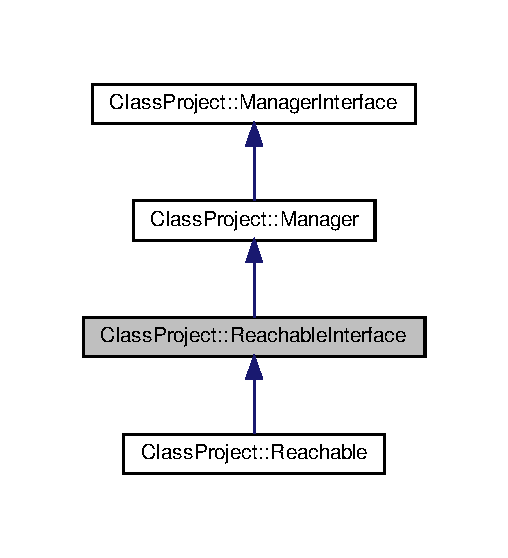
\includegraphics[width=244pt]{classClassProject_1_1ReachableInterface__inherit__graph}
\end{center}
\end{figure}


Collaboration diagram for Class\+Project\+:\+:Reachable\+Interface\+:
\nopagebreak
\begin{figure}[H]
\begin{center}
\leavevmode
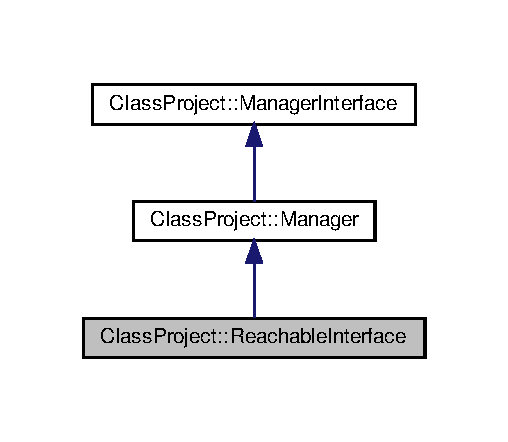
\includegraphics[width=244pt]{classClassProject_1_1ReachableInterface__coll__graph}
\end{center}
\end{figure}
\subsection*{Public Member Functions}
\begin{DoxyCompactItemize}
\item 
\hyperlink{classClassProject_1_1ReachableInterface_a80afbca3170ebe434924fb7625cc9025}{Reachable\+Interface} (unsigned int state\+Size)
\item 
\mbox{\Hypertarget{classClassProject_1_1ReachableInterface_ac6d3bf3f4b98c775a944053f3dbffd69}\label{classClassProject_1_1ReachableInterface_ac6d3bf3f4b98c775a944053f3dbffd69}} 
virtual unsigned int {\bfseries return\+\_\+state\+Size} ()
\item 
virtual B\+D\+D\+\_\+\+ID \hyperlink{classClassProject_1_1ReachableInterface_a80163dcb8b1d982b4fb7f8614808dece}{xnor2} (B\+D\+D\+\_\+\+ID a, B\+D\+D\+\_\+\+ID b)=0
\item 
virtual const std\+::vector$<$ B\+D\+D\+\_\+\+ID $>$ \& \hyperlink{classClassProject_1_1ReachableInterface_a8546499fbc6d0da61b6b21f8db8e4621}{get\+States} () const =0
\item 
virtual void \hyperlink{classClassProject_1_1ReachableInterface_a88f9a34f7272c3f971e757aa2b140746}{set\+Delta} (const std\+::vector$<$ B\+D\+D\+\_\+\+ID $>$ \&transition\+Functions)=0
\item 
virtual void \hyperlink{classClassProject_1_1ReachableInterface_a005d8d8375b8d4e9f7c7d1a0ff01a97f}{set\+Init\+State} (const std\+::vector$<$ bool $>$ \&state\+Vector)=0
\item 
virtual B\+D\+D\+\_\+\+ID \hyperlink{classClassProject_1_1ReachableInterface_a84a2fe53f724c184266fc22f17204499}{compute\+\_\+reachable\+\_\+states} ()=0
\item 
virtual bool \hyperlink{classClassProject_1_1ReachableInterface_aa3011f06562431832cf563b77fb36c13}{is\+\_\+reachable} (const std\+::vector$<$ bool $>$ \&state\+Vector)=0
\end{DoxyCompactItemize}


\subsection{Detailed Description}
Defines the implemented interface of the reachability extension. 

\subsection{Constructor \& Destructor Documentation}
\mbox{\Hypertarget{classClassProject_1_1ReachableInterface_a80afbca3170ebe434924fb7625cc9025}\label{classClassProject_1_1ReachableInterface_a80afbca3170ebe434924fb7625cc9025}} 
\index{Class\+Project\+::\+Reachable\+Interface@{Class\+Project\+::\+Reachable\+Interface}!Reachable\+Interface@{Reachable\+Interface}}
\index{Reachable\+Interface@{Reachable\+Interface}!Class\+Project\+::\+Reachable\+Interface@{Class\+Project\+::\+Reachable\+Interface}}
\subsubsection{\texorpdfstring{Reachable\+Interface()}{ReachableInterface()}}
{\footnotesize\ttfamily Class\+Project\+::\+Reachable\+Interface\+::\+Reachable\+Interface (\begin{DoxyParamCaption}\item[{unsigned int}]{state\+Size }\end{DoxyParamCaption})\hspace{0.3cm}{\ttfamily [inline]}, {\ttfamily [explicit]}}

Constructor creates state\+Size state bits for the user 
\begin{DoxyParams}{Parameters}
{\em state\+Size} & state size \\
\hline
\end{DoxyParams}


\subsection{Member Function Documentation}
\mbox{\Hypertarget{classClassProject_1_1ReachableInterface_a84a2fe53f724c184266fc22f17204499}\label{classClassProject_1_1ReachableInterface_a84a2fe53f724c184266fc22f17204499}} 
\index{Class\+Project\+::\+Reachable\+Interface@{Class\+Project\+::\+Reachable\+Interface}!compute\+\_\+reachable\+\_\+states@{compute\+\_\+reachable\+\_\+states}}
\index{compute\+\_\+reachable\+\_\+states@{compute\+\_\+reachable\+\_\+states}!Class\+Project\+::\+Reachable\+Interface@{Class\+Project\+::\+Reachable\+Interface}}
\subsubsection{\texorpdfstring{compute\+\_\+reachable\+\_\+states()}{compute\_reachable\_states()}}
{\footnotesize\ttfamily virtual B\+D\+D\+\_\+\+ID Class\+Project\+::\+Reachable\+Interface\+::compute\+\_\+reachable\+\_\+states (\begin{DoxyParamCaption}{ }\end{DoxyParamCaption})\hspace{0.3cm}{\ttfamily [pure virtual]}}

Computes the symbolic representation of the reachable states. Before this method is called it is important to set the transition function and the initial state. \begin{DoxyReturn}{Returns}
B\+D\+D\+\_\+\+ID of the reachable state space 
\end{DoxyReturn}


Implemented in \hyperlink{classClassProject_1_1Reachable_ab382d204af0fe91f027026b6dad6142f}{Class\+Project\+::\+Reachable}.

\mbox{\Hypertarget{classClassProject_1_1ReachableInterface_a8546499fbc6d0da61b6b21f8db8e4621}\label{classClassProject_1_1ReachableInterface_a8546499fbc6d0da61b6b21f8db8e4621}} 
\index{Class\+Project\+::\+Reachable\+Interface@{Class\+Project\+::\+Reachable\+Interface}!get\+States@{get\+States}}
\index{get\+States@{get\+States}!Class\+Project\+::\+Reachable\+Interface@{Class\+Project\+::\+Reachable\+Interface}}
\subsubsection{\texorpdfstring{get\+States()}{getStates()}}
{\footnotesize\ttfamily virtual const std\+::vector$<$B\+D\+D\+\_\+\+ID$>$\& Class\+Project\+::\+Reachable\+Interface\+::get\+States (\begin{DoxyParamCaption}{ }\end{DoxyParamCaption}) const\hspace{0.3cm}{\ttfamily [pure virtual]}}

States are generated and stored in a vector. These lsb (e.\+g. \char`\"{}s0\char`\"{}) is stored at location 0. The msb(e.\+g. \char`\"{}s3\char`\"{}) is stored at location size-\/1. \begin{DoxyReturn}{Returns}
vector with the B\+D\+D\+\_\+\+ID of each state bit 
\end{DoxyReturn}


Implemented in \hyperlink{classClassProject_1_1Reachable_a46b6aab8ea4dac374af4e2e97b5321dd}{Class\+Project\+::\+Reachable}.

\mbox{\Hypertarget{classClassProject_1_1ReachableInterface_aa3011f06562431832cf563b77fb36c13}\label{classClassProject_1_1ReachableInterface_aa3011f06562431832cf563b77fb36c13}} 
\index{Class\+Project\+::\+Reachable\+Interface@{Class\+Project\+::\+Reachable\+Interface}!is\+\_\+reachable@{is\+\_\+reachable}}
\index{is\+\_\+reachable@{is\+\_\+reachable}!Class\+Project\+::\+Reachable\+Interface@{Class\+Project\+::\+Reachable\+Interface}}
\subsubsection{\texorpdfstring{is\+\_\+reachable()}{is\_reachable()}}
{\footnotesize\ttfamily virtual bool Class\+Project\+::\+Reachable\+Interface\+::is\+\_\+reachable (\begin{DoxyParamCaption}\item[{const std\+::vector$<$ bool $>$ \&}]{state\+Vector }\end{DoxyParamCaption})\hspace{0.3cm}{\ttfamily [pure virtual]}}

This method decides whether a specific state is in the reachable state space or not. The inpute is provided as a vector of states. The value is true if the state bit is high in this state, false otherwise. 
\begin{DoxyParams}{Parameters}
{\em state\+Vector} & \\
\hline
\end{DoxyParams}
\begin{DoxyReturn}{Returns}

\end{DoxyReturn}


Implemented in \hyperlink{classClassProject_1_1Reachable_a19a40b477fc119690e0a9f1f7ffc4843}{Class\+Project\+::\+Reachable}.

\mbox{\Hypertarget{classClassProject_1_1ReachableInterface_a88f9a34f7272c3f971e757aa2b140746}\label{classClassProject_1_1ReachableInterface_a88f9a34f7272c3f971e757aa2b140746}} 
\index{Class\+Project\+::\+Reachable\+Interface@{Class\+Project\+::\+Reachable\+Interface}!set\+Delta@{set\+Delta}}
\index{set\+Delta@{set\+Delta}!Class\+Project\+::\+Reachable\+Interface@{Class\+Project\+::\+Reachable\+Interface}}
\subsubsection{\texorpdfstring{set\+Delta()}{setDelta()}}
{\footnotesize\ttfamily virtual void Class\+Project\+::\+Reachable\+Interface\+::set\+Delta (\begin{DoxyParamCaption}\item[{const std\+::vector$<$ B\+D\+D\+\_\+\+ID $>$ \&}]{transition\+Functions }\end{DoxyParamCaption})\hspace{0.3cm}{\ttfamily [pure virtual]}}

Each state variable has a transition function. The transition function specifies the value of the state after the transition. The transition function are composed of only state variables. For example\+: s0\textquotesingle{} = s0 X\+OR s1 The next state is defined as X\+OR of the current values of the state bit s0 and s1 
\begin{DoxyParams}{Parameters}
{\em transition\+Functions} & provide a transition function exactly for each state bit \\
\hline
\end{DoxyParams}


Implemented in \hyperlink{classClassProject_1_1Reachable_a53fdcc94c37cd7f0e27881678189b5c5}{Class\+Project\+::\+Reachable}.

\mbox{\Hypertarget{classClassProject_1_1ReachableInterface_a005d8d8375b8d4e9f7c7d1a0ff01a97f}\label{classClassProject_1_1ReachableInterface_a005d8d8375b8d4e9f7c7d1a0ff01a97f}} 
\index{Class\+Project\+::\+Reachable\+Interface@{Class\+Project\+::\+Reachable\+Interface}!set\+Init\+State@{set\+Init\+State}}
\index{set\+Init\+State@{set\+Init\+State}!Class\+Project\+::\+Reachable\+Interface@{Class\+Project\+::\+Reachable\+Interface}}
\subsubsection{\texorpdfstring{set\+Init\+State()}{setInitState()}}
{\footnotesize\ttfamily virtual void Class\+Project\+::\+Reachable\+Interface\+::set\+Init\+State (\begin{DoxyParamCaption}\item[{const std\+::vector$<$ bool $>$ \&}]{state\+Vector }\end{DoxyParamCaption})\hspace{0.3cm}{\ttfamily [pure virtual]}}

Each state machine has an inital state. The inital state is provided as a vector. The vector has to have an entry for each state bit. If the entry is \char`\"{}true\char`\"{} the state bit is high, otherwhise negated. E.\+g. initial state not(s0) and not(s1) is transformed into \{false,false\}. 
\begin{DoxyParams}{Parameters}
{\em state\+Vector} & provide the assignemtn for each state bit \\
\hline
\end{DoxyParams}


Implemented in \hyperlink{classClassProject_1_1Reachable_ab3ddc3f569e280c3902a40ab8202f8c3}{Class\+Project\+::\+Reachable}.

\mbox{\Hypertarget{classClassProject_1_1ReachableInterface_a80163dcb8b1d982b4fb7f8614808dece}\label{classClassProject_1_1ReachableInterface_a80163dcb8b1d982b4fb7f8614808dece}} 
\index{Class\+Project\+::\+Reachable\+Interface@{Class\+Project\+::\+Reachable\+Interface}!xnor2@{xnor2}}
\index{xnor2@{xnor2}!Class\+Project\+::\+Reachable\+Interface@{Class\+Project\+::\+Reachable\+Interface}}
\subsubsection{\texorpdfstring{xnor2()}{xnor2()}}
{\footnotesize\ttfamily virtual B\+D\+D\+\_\+\+ID Class\+Project\+::\+Reachable\+Interface\+::xnor2 (\begin{DoxyParamCaption}\item[{B\+D\+D\+\_\+\+ID}]{a,  }\item[{B\+D\+D\+\_\+\+ID}]{b }\end{DoxyParamCaption})\hspace{0.3cm}{\ttfamily [pure virtual]}}

\begin{DoxyReturn}{Returns}
returns the X\+N\+OR of B\+DD I\+Ds 
\end{DoxyReturn}


Implemented in \hyperlink{classClassProject_1_1Reachable_a7f97f9868c825b64f333c4bc8eb7632b}{Class\+Project\+::\+Reachable}.


\hypertarget{structClassProject_1_1uTableVal}{}\section{Class\+Project\+:\+:u\+Table\+Val Struct Reference}
\label{structClassProject_1_1uTableVal}\index{Class\+Project\+::u\+Table\+Val@{Class\+Project\+::u\+Table\+Val}}


Struct used as value in the unique table.  




{\ttfamily \#include $<$Manager.\+h$>$}

\subsection*{Public Member Functions}
\begin{DoxyCompactItemize}
\item 
\mbox{\Hypertarget{structClassProject_1_1uTableVal_a63378667dd6920a1d6ab2831eab7d17f}\label{structClassProject_1_1uTableVal_a63378667dd6920a1d6ab2831eab7d17f}} 
{\bfseries u\+Table\+Val} (B\+D\+D\+\_\+\+ID \+\_\+highV, B\+D\+D\+\_\+\+ID \+\_\+lowV, B\+D\+D\+\_\+\+ID \+\_\+top\+Var)
\end{DoxyCompactItemize}
\subsection*{Public Attributes}
\begin{DoxyCompactItemize}
\item 
\mbox{\Hypertarget{structClassProject_1_1uTableVal_aec6c964e6a8284ff09eba51260548126}\label{structClassProject_1_1uTableVal_aec6c964e6a8284ff09eba51260548126}} 
B\+D\+D\+\_\+\+ID {\bfseries highV}
\item 
\mbox{\Hypertarget{structClassProject_1_1uTableVal_a69dc988fc82c3d96902402fa6247ec22}\label{structClassProject_1_1uTableVal_a69dc988fc82c3d96902402fa6247ec22}} 
B\+D\+D\+\_\+\+ID {\bfseries lowV}
\item 
\mbox{\Hypertarget{structClassProject_1_1uTableVal_ab659596f0cc616efd1cb43f14b6a1bd2}\label{structClassProject_1_1uTableVal_ab659596f0cc616efd1cb43f14b6a1bd2}} 
B\+D\+D\+\_\+\+ID {\bfseries top\+Var}
\end{DoxyCompactItemize}


\subsection{Detailed Description}
Struct used as value in the unique table. 

This data structure contains the corresponding information of a node in the unique table of the B\+DD (excluding its ID, which comes aside). It includes the following elements\+:
\begin{DoxyItemize}
\item High\+: ID of the node representing the positive cofactor.
\item Low\+: ID of the node representing the negative cofactor.
\item Top variable\+: ID of the top variable reachable from the node. 
\end{DoxyItemize}
%--- End generated contents ---

% Index
\backmatter
\newpage
\phantomsection
\clearemptydoublepage
\addcontentsline{toc}{chapter}{Index}
\printindex

\end{document}
